\subsection{Dissecting the Differential IFIT2 Antibody Staining} \label{subsec:Dissecting the Differential IFIT2 Antibody Staining}
In Chapter \ref{ch:Subcellular Localisation of Endogenous IFIT Proteins in the Context of RSV Inclusion Bodies} we have observed a strinking differential staining patternt between the two utilised anti-IFIT2 antibodies with regards to the observed interaction of IFIT with human or bovine RSV inclusion bodies. IFIT2(A) antibody showed both human and bovine IFIT2 to form intra-IB inclusions in smaller IBs, while it has observed IFIT2 to colocalise with the IB edge while being excluded from the IB centre of larger IBs. IFIT2(B) on the other hand predominantly detected IFIT2 to be excluded from the IB structures, indiscriminantly of the IB size. It has also occasionally showed IFIT2 to be equally distributed between the cytoplasm and the IB structures. Along to these, we have also observed a differenatial stainng pattern with regards to the general subcellular localisation of IFIT2 in mock-treated cells, which was more pronounced in the bovine cells. While we have observed general cytoplasmic staining of bovine IFIT2 by both antibodies, the IFIT2(A) staning alo revealed perinuclear concentations, which resemble the golgi aparatus. On the other hand, the IFIT2(B) antibody revealed IFIT2 to colocalise with the mitotic spindle. Clearly it seems like these two polyclonal antibodies are detecting two different entities. We believe these are two populations of IFIT2, basaly present in both human and bovine cells which are being detected by the antibodies based on differential epitope detecton. This could be due to one antibody detecting IFIT2 in the complex of its interaction partners such as IFIT1, IFIT3, MAVS, HOMER3, or double-strandeed RNA, while the other antibody detects naked IFIT2 entities. The precise nature, however, still remains to be elucitaded.

To iunvestigate this we initialy employed the same methodologies as were used in Section \ref{subsec:IFIT1, IFIT3, and IFIT5 Localisation with Regards to RSV Pseudo-IBs} i.e. we set to investigate the IFIT2 localisation with regards to human and bovine RSV pIBs, as detected by the IFIT2(A) and IFIT2(B) antibodies. We have utilised the HEK293T and Vero cell lines in which we probed for endogenous human and monkey IFIT2 respectively. We have induced hRSV pIBs in both HEK293T, and Vero cell lines utilising the transfection pcDNA3.1 plasmids containing ORFs for hRSV \textit{N} and \textit{P}, while have assessed the bRSV pIBs solely in Vero cell line. We have however failed to generate sufficient amounbt of bRSV pIB expressiing Vero cells to stain with both IFIT2(A) and IFIT2(B) andtibodies and thus the latter is missiing from the analysis. This could be due to contaminations in the plasmid preperations or decreased quality of these plasmids.

\begin{figure}
    \centering
    \includegraphics[width=1\linewidth]{09. Chapter 4/Figs/01. pIB/03. IFIT2/01. Single Transfection/01. 293t-ifit2a.pdf}
    \caption[IFIT2(A) Antibody Detects Increased IFIT2 Expression Following hRSV P Transfection.]{\textbf{IFIT2(A) Antibody Detects Increased IFIT2 Expression Following hRSV P Transfection.} HEK293T cells were either mock transfected, or single transfected with empty vector, hRSV N containing plasmid, or hRSV P containing plasmid using TransIT-X2 and were fixed after 24 hours. Cellular nuclei were stained with DAPI (yellow), and cells were double-labelled with either anti-RSV N (cyan), or anti-RSV P (cyan) and anti-IFIT2(A) (magenta) antibodies. The scale bar indicates 50 \(\mu \mbox{m}\).}
    \label{fig:IFIT2(A) Antibody Detects Increased IFIT2 Expression Following hRSV P Transfection}
\end{figure}

\begin{figure}
    \centering
    \includegraphics[width=1\linewidth]{09. Chapter 4/Figs/01. pIB/03. IFIT2/01. Single Transfection/02. 293t-ifit2b.pdf}
    \caption[IFIT2(B) Antibody Does Not Detect Increased IFIT2 Expression Following hRSV P Transfection.]{\textbf{IFIT2(B) Antibody Does Not Detect Increased IFIT2 Expression Following hRSV P Transfection.} HEK293T cells were either mock transfected, or single transfected with empty vector, hRSV N containing plasmid, or hRSV P containing plasmid using TransIT-X2 and were fixed after 24 hours. Cellular nuclei were stained with DAPI (yellow), and cells were double-labelled with either anti-RSV N (cyan), or anti-RSV P (cyan) and anti-IFIT2(B) (magenta) antibodies. The scale bar indicates 50 \(\mu \mbox{m}\).}
    \label{fig:IFIT2(B) Antibody Does Not Detect Increased IFIT2 Expression Following hRSV P Transfection}
\end{figure}

While conducting the fundemental control experiments consisting of asssesing the single RSV \textit{N} and \textit{P} transfectons, along with transfections with empty pcDNA3.1 plasmid, while comparing these to mock-transfected cells we have uncovered another differentiation between IFIT2(A) and IFIT2(B) staining. We have observed IFIT2 induction as a response to transfection with hRSV \textit{P}-containing plasmid, which did not occur during the transfection with empty vector or hRSV \textit{N}-containing plasmid. This induction occured only in the cells where we dected hRSV \textit{P} expression. Interesingly, this was only detected using IFIT2(A) (Figure \ref{fig:IFIT2(A) Antibody Detects Increased IFIT2 Expression Following hRSV P Transfection}), while IFIT2(B) staining did not revel this phenotype (Figure \ref{fig:IFIT2(B) Antibody Does Not Detect Increased IFIT2 Expression Following hRSV P Transfection}). We conducted these control experiments for IFIT1, IFIT3, and IFIT5 which revealed staining patter consistent to what IFIT2(B) antibody observed (data not shown). Along to this, we can observe differential subcellular localisation of IFIT2 between the detection of the two antibodies, which is somewhat consistent to what was observed in Chapter \ref{ch:Subcellular Localisation of Endogenous IFIT Proteins in the Context of RSV Inclusion Bodies} in the MDBK cell line. We have observed IFIT2(A)-stained HEK293T mock cells to show perinuclear IFT2 concentrations resembling lipid droplets or aggregosomes, based the definitions and expamples provided by the Human Protien Atlas \cite{Thul2017AProteome}. The IFIT2(B) antibody showed IFIT2 localising to the mitotic spindle. This data poses a few questions. Since the \textit{IFIT} genes should possess similar genomic regulation, through which mechanism does \textit{IFIT2} get induced following RSV \textit{P} exogenous expression? Is this mediated via the direct acxtion of the P protein and thus is this indicative to what happens during infection? This would imply that the \textit{hIFIT2} induction caused by RSV infection (from Chapter \ref{ch:Assessment of Transcriptional Induction of Human IFITs in the Context of RSV}) apperas predominantly in infected, P expressing cells and thus hnts at direct IFIT2 antiviral role against RSV. The other imnportant question is how is it possible that IFIT2(B) antibody is unable to detect this increased nascent IFIT2? If the previously mentioned differential target epitope, based on the IFIT2 interaction partners is correct, this would suggest that IFIT2(B) antibody detects IFIT2 complexes and thus is blind to the newly synthesised IFIT2, which did not have time to for this complexes yet. Further expreiments are required to validate this claim.

\begin{figure}
    \begin{subfigure}{0.495\textwidth}
        \caption{}
        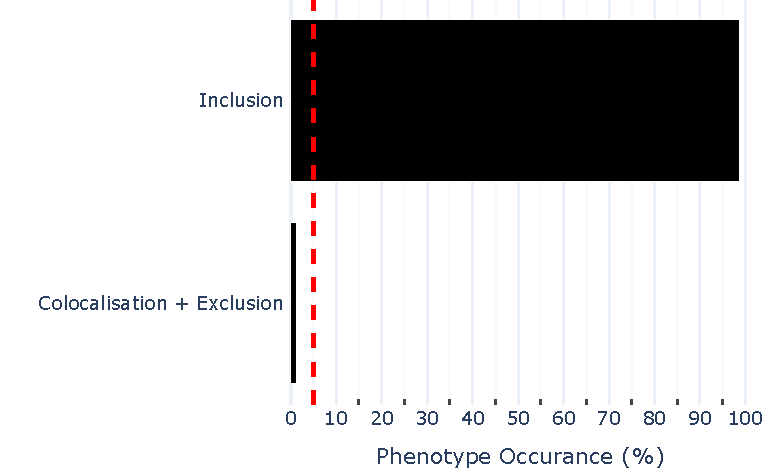
\includegraphics[width=1\linewidth]{09. Chapter 4/Figs/01. pIB/03. IFIT2/02. IFIT2A/01. bar_i2a_293t.pdf}
    \end{subfigure}
    \begin{subfigure}{0.495\textwidth}
        \caption{}
        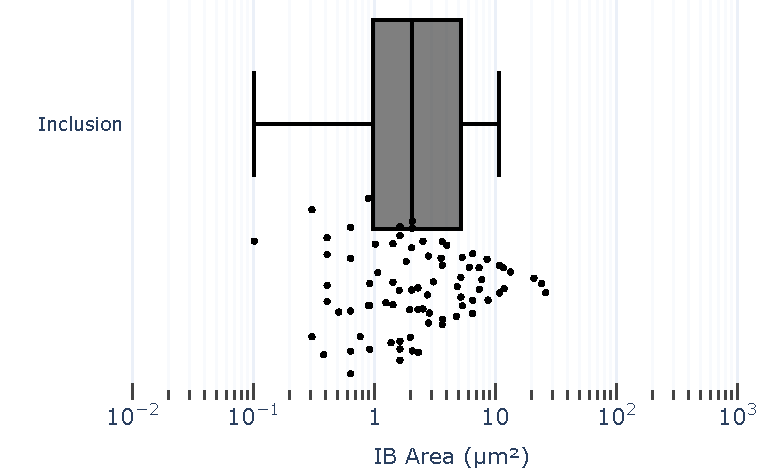
\includegraphics[width=1\linewidth]{09. Chapter 4/Figs/01. pIB/03. IFIT2/02. IFIT2A/02. box_i2a_293t.pdf}
    \end{subfigure}
    \caption[Observed Phenotypes of Endogenous Human IFIT2 in the Context of hRSV Pseudo Inclusion Bodies in 293T Cell Line, as Detected by IFIT2(A) Antibody.]{\textbf{Observed Phenotypes of Endogenous Human IFIT2 in the Context of hRSV Pseudo Inclusion Bodies in 293T Cell Line, as Detected by IFIT2(A) Antibody.} 293T cells were transfected with hRSV N and P containing plasmids using TransIT-X2 and were fixed after 24 hours. Cells were labelled with anti-RSV N and anti-IFIT2(A) antibodies and imaged on a confocal microscope. Panel (a) shows the percentual proportions of observed phenotypes between hRSV pseudo inclusion bodies and human IFIT2 (81 observations), with the red dotted line denoting the 5\% threshold, marking phenotypes considered relevant above this limit. Panel (b) shows the IB area in \(\mu \mbox{m}^2\) per observed relevant phenotype.}
    \label{fig:Observed Phenotypes of Endogenous Human IFIT2 in the Context of hRSV Pseudo Inclusion Bodies in 293T Cell Line, as Detected by IFIT2(A) Antibody}
\end{figure}

\begin{figure}
    \centering
    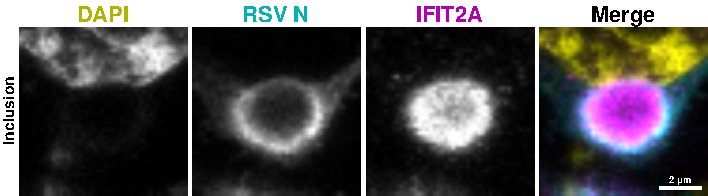
\includegraphics[width=1\linewidth]{09. Chapter 4/Figs/01. pIB/03. IFIT2/02. IFIT2A/03. i2a-293t-hnhp.pdf} 
    \caption[Representative Images of Observed Phenotypes of Endogenous Human IFIT2 in the Context of hRSV Pseudo Inclusion Bodies in 293T Cell Line, as Detected by IFIT2(A) Antibody.]{\textbf{Representative Images of Observed Phenotypes of Endogenous Human IFIT2 in the Context of hRSV Pseudo Inclusion Bodies in 293T Cell Line, as Detected by IFIT2(A) Antibody.} 293T cells were transfected with hRSV N and P containing plasmids using TransIT-X2 and were fixed after 24 hours. Cellular nuclei were stained with DAPI (yellow), and cells were double-labelled with anti-RSV N (cyan) and anti-IFIT2(A) (magenta) antibodies. This figure showcases representative examples of relevant phenotypes in the interaction between human IFIT2 and hRSV pseudo-inclusion bodies. These phenotypes are presented in descending order based on their percentage proportions. The scale bar indicates 2 \(\mu \mbox{m}\).}
    \label{fig:Representative Images of Observed Phenotypes of Endogenous Human IFIT2 in the Context of hRSV Pseudo Inclusion Bodies in 293T Cell Line, as Detected by IFIT2(A) Antibody}
\end{figure}

Next, we set to investigate the interaction phenotypes of IFIT2 with RSV pseudo IBs as detected by the two antibodies, firstly focusing on the signal detected by IFIT2(A) antibody. We have obtained 81 observation of human IFIT2 interacting with hRSV pIBs from HEK293T cell line. The observed phenotypes, along with their frequencies of occurances and the pIB sizes associated with phenotypic interactions that occur with higher than 5\% frequency are shown in Figure \ref{fig:Observed Phenotypes of Endogenous Human IFIT2 in the Context of hRSV Pseudo Inclusion Bodies in 293T Cell Line, as Detected by IFIT2(A) Antibody}, with the represpentaitve images of the phenotypes occuring at more than 5\% frequency are shown in Figure \ref{fig:Representative Images of Observed Phenotypes of Endogenous Human IFIT2 in the Context of hRSV Pseudo Inclusion Bodies in 293T Cell Line, as Detected by IFIT2(A) Antibody}. predominantly we have observed IFIT2 to form intra-pIB inclusion, a phenotype that occur in 98\% of cases. In the remaining 2\% of observations we have observed IFIT2 colocalising with the pIB boundry, while being excluded form the pIB centre. The sizes of inclusion-associated pIBs confront to the general distribution of all obsebserved pIBs in HEK293T cell line, ranging from 0.1 \(\mu \mbox{m}^2\) to 25 \(\mu \mbox{m}^2\) in size, with the median area of 2 \(\mu \mbox{m}^2\). Unlike what we observed with monkey IFIT1 and IFIT5, where the inclusion and colocalisation associated with exclusion phenotypes seem to be restricted to small and large pIBs respectively, we do not see this discintion with endogenous human IFIT2. This suggest that IFIT2, as detected by IFIT2(A) antibody seems to form intra-pIB inclusions, irrespective of their size.

\begin{figure}
    \begin{subfigure}{0.495\textwidth}
        \caption{}
        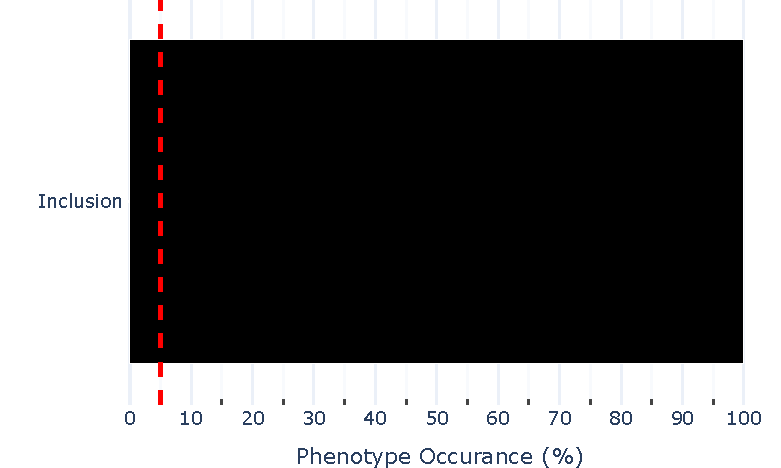
\includegraphics[width=1\linewidth]{09. Chapter 4/Figs/01. pIB/03. IFIT2/02. IFIT2A/04. bar_i2a_vero_hnhp.pdf} 
    \end{subfigure}
    \begin{subfigure}{0.495\textwidth}
        \caption{}
        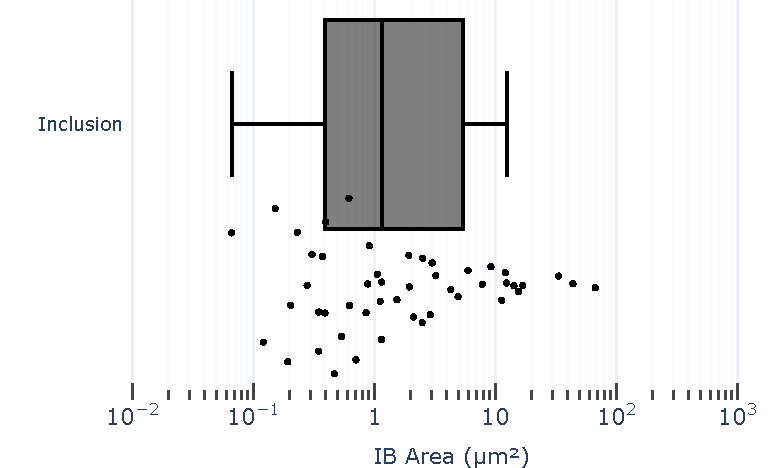
\includegraphics[width=1\linewidth]{09. Chapter 4/Figs/01. pIB/03. IFIT2/02. IFIT2A/05. box_i2a_vero_hnhp.pdf}
    \end{subfigure}
    \caption[Observed Phenotypes of Endogenous Monkey IFIT2 in the Context of hRSV Pseudo Inclusion Bodies in Vero Cell Line, as Detected by IFIT2(A) Antibody.]{\textbf{Observed Phenotypes of Endogenous Monkey IFIT2 in the Context of hRSV Pseudo Inclusion Bodies in Vero Cell Line, as Detected by IFIT2(A) Antibody.} Vero cells were transfected with hRSV N and P containing plasmids using TransIT-X2 and were fixed after 24 hours. Cells were labelled with anti-RSV N and anti-IFIT2(A) antibodies and imaged on a confocal microscope. Panel (a) shows the percentual proportions of observed phenotypes between hRSV pseudo inclusion bodies and monkey IFIT2 (48 observations), with the red dotted line denoting the 5\% threshold, marking phenotypes considered relevant above this limit. Panel (b) shows the IB area in \(\mu \mbox{m}^2\) per observed relevant phenotype.}
    \label{fig:Observed Phenotypes of Endogenous Monkey IFIT2 in the Context of hRSV Pseudo Inclusion Bodies in Vero Cell Line, as Detected by IFIT2(A) Antibody}
\end{figure}

\begin{figure}
    \centering
    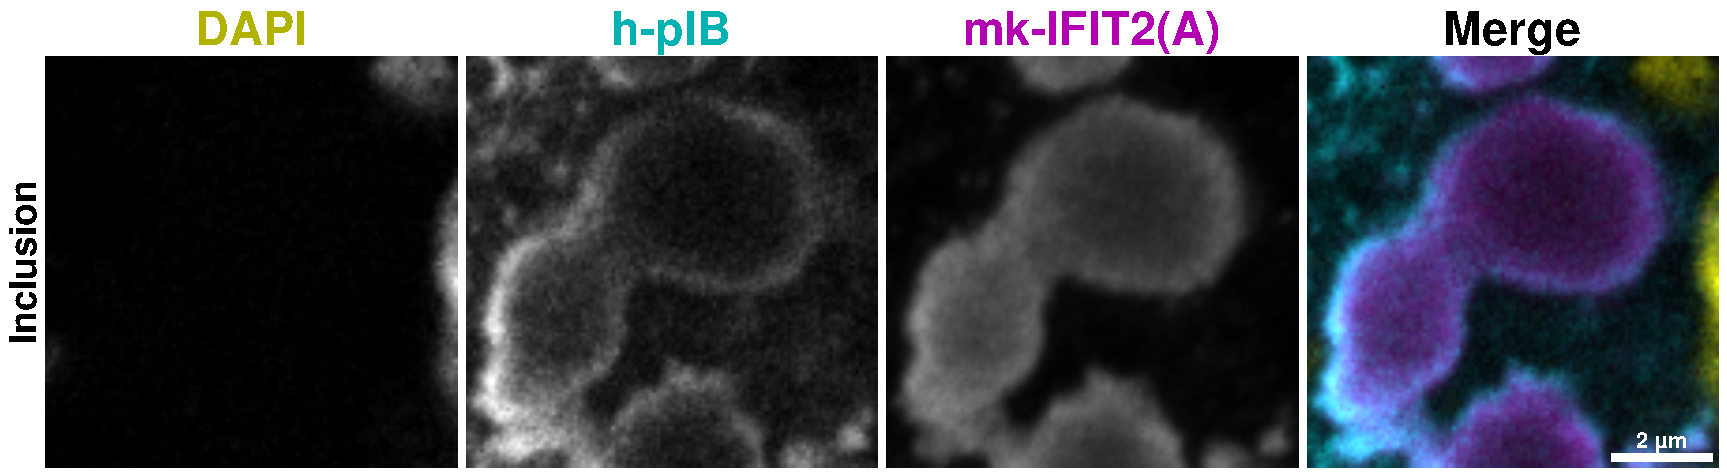
\includegraphics[width=1\linewidth]{09. Chapter 4/Figs/01. pIB/03. IFIT2/02. IFIT2A/06. i2a-vero-hnhp.pdf}  
    \caption[Representative Images of Observed Phenotypes of Endogenous Monkey IFIT2 in the Context of hRSV Pseudo Inclusion Bodies in Vero Cell Line, as Detected by IFIT2(A) Antibody.]{\textbf{Representative Images of Observed Phenotypes of Endogenous Monkey IFIT2 in the Context of hRSV Pseudo Inclusion Bodies in Vero Cell Line, as Detected by IFIT2(A) Antibody.} Vero cells were transfected with hRSV N and P containing plasmids using TransIT-X2 and were fixed after 24 hours. Cellular nuclei were stained with DAPI (yellow), and cells were double-labelled with anti-RSV N (cyan) and anti-IFIT2(A) (magenta) antibodies. This figure showcases representative examples of relevant phenotypes in the interaction between monkey IFIT2 and hRSV pseudo-inclusion bodies. These phenotypes are presented in descending order based on their percentage proportions. The scale bar indicates 2 \(\mu \mbox{m}\).}
    \label{fig:Representative Images of Observed Phenotypes of Endogenous Monkey IFIT2 in the Context of hRSV Pseudo Inclusion Bodies in Vero Cell Line, as Detected by IFIT2(A) Antibody}
\end{figure}

Next we investigated the monkey IFIT2 interaction with hRSV pIBs as detected by the IFIT2(A) antibody. To do this we trnasfected hRSV \textit{N} and \textit{P} containing plasmids to Vero cells. Doing this we have obtained 48 observations, all of which confronted to the inclusion phyenotype (Figure \ref{fig:Observed Phenotypes of Endogenous Monkey IFIT2 in the Context of hRSV Pseudo Inclusion Bodies in Vero Cell Line, as Detected by IFIT2(A) Antibody}, panel a). The measured area of these hRSV pIBs is showin in Figure \ref{fig:Observed Phenotypes of Endogenous Monkey IFIT2 in the Context of hRSV Pseudo Inclusion Bodies in Vero Cell Line, as Detected by IFIT2(A) Antibody}, panel b. The representative image is shown in Figure \ref{fig:Representative Images of Observed Phenotypes of Endogenous Monkey IFIT2 in the Context of hRSV Pseudo Inclusion Bodies in Vero Cell Line, as Detected by IFIT2(A) Antibody}. The distribution of the pIB sizes is almost indentical to the aggregate dataset of all pIBs observed in Vero cell line, ranging from sub 0.07 \(\mu \mbox{m}^2\) to supra 60 \(\mu \mbox{m}^2\), with the typical value of 1.2 \(\mu \mbox{m}^2\). This data is consistent to what we observed in HEK293T cells. 

\begin{figure}
    \begin{subfigure}{0.495\textwidth}
        \caption{}
        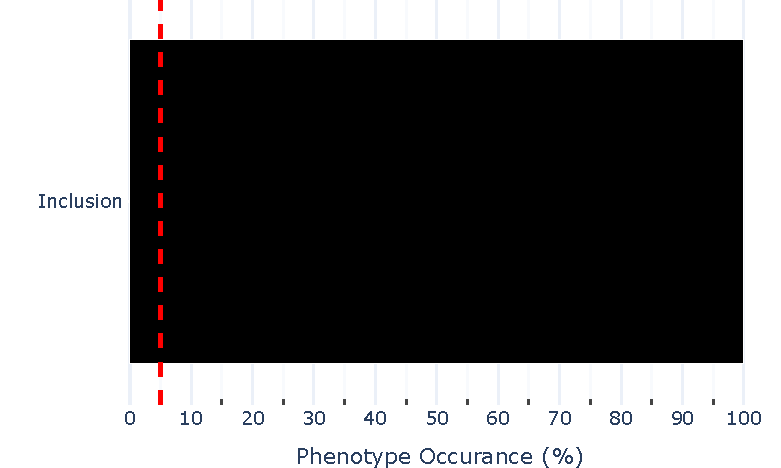
\includegraphics[width=1\linewidth]{09. Chapter 4/Figs/01. pIB/03. IFIT2/02. IFIT2A/07. bar_i2a_vero_bnbp.pdf} 
    \end{subfigure}
    \begin{subfigure}{0.495\textwidth}
        \caption{}
        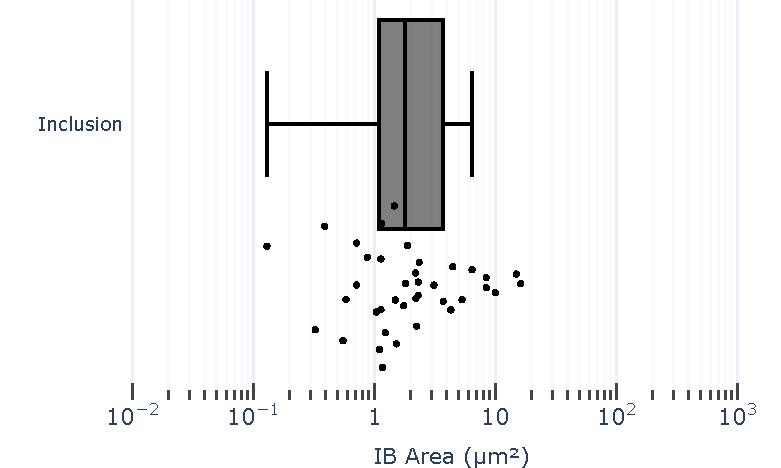
\includegraphics[width=1\linewidth]{09. Chapter 4/Figs/01. pIB/03. IFIT2/02. IFIT2A/08. box_i2a_vero_bnbp.pdf}
    \end{subfigure}
    \caption[Observed Phenotypes of Endogenous Monkey IFIT2 in the Context of bRSV Pseudo Inclusion Bodies in Vero Cell Line, as Detected by IFIT2(A) Antibody.]{\textbf{Observed Phenotypes of Endogenous Monkey IFIT2 in the Context of bRSV Pseudo Inclusion Bodies in Vero Cell Line, as Detected by IFIT2(A) Antibody.} Vero cells were transfected with bRSV N and P containing plasmids using TransIT-X2 and were fixed after 24 hours. Cells were labelled with anti-RSV N and anti-IFIT2(A) antibodies and imaged on a confocal microscope. Panel (a) shows the percentual proportions of observed phenotypes between bRSV pseudo inclusion bodies and monkey IFIT2 (38 observations), with the red dotted line denoting the 5\% threshold, marking phenotypes considered relevant above this limit. Panel (b) shows the IB area in \(\mu \mbox{m}^2\) per observed relevant phenotype.}
    \label{fig:Observed Phenotypes of Endogenous Monkey IFIT2 in the Context of bRSV Pseudo Inclusion Bodies in Vero Cell Line, as Detected by IFIT2(A) Antibody}
\end{figure}

\begin{figure}
    \centering
    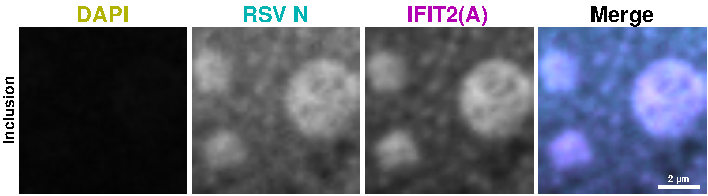
\includegraphics[width=1\linewidth]{09. Chapter 4/Figs/01. pIB/03. IFIT2/02. IFIT2A/09. i2a-vero-bnbp.pdf} 
    \caption[Representative Images of Observed Phenotypes of Endogenous Monkey IFIT2 in the Context of bRSV Pseudo Inclusion Bodies in Vero Cell Line, as Detected by IFIT2(A) Antibody.]{\textbf{Representative Images of Observed Phenotypes of Endogenous Monkey IFIT2 in the Context of bRSV Pseudo Inclusion Bodies in Vero Cell Line, as Detected by IFIT2(A) Antibody.} Vero cells were transfected with bRSV N and P containing plasmids using TransIT-X2 and were fixed after 24 hours. Cellular nuclei were stained with DAPI (yellow), and cells were double-labelled with anti-RSV N (cyan) and anti-IFIT2(A) (magenta) antibodies. This figure showcases representative examples of relevant phenotypes in the interaction between monkey IFIT2 and bRSV pseudo-inclusion bodies. These phenotypes are presented in descending order based on their percentage proportions. The scale bar indicates 2 \(\mu \mbox{m}\).}
    \label{fig:Representative Images of Observed Phenotypes of Endogenous Monkey IFIT2 in the Context of bRSV Pseudo Inclusion Bodies in Vero Cell Line, as Detected by IFIT2(A) Antibody}
\end{figure}

Finally we investigated the monkey IFIT2 interaction with bRSV pIBs as detected by the IFIT2(A) antibody. To do this we trnasfected bRSV \textit{N} and \textit{P} containing plasmids to Vero cells. Doing this we have obtained 38 observations, all of which confronted to the inclusion phyenotype (Figure \ref{fig:Observed Phenotypes of Endogenous Monkey IFIT2 in the Context of bRSV Pseudo Inclusion Bodies in Vero Cell Line, as Detected by IFIT2(A) Antibody}, panel a). The measured area of these bRSV pIBs is showin in Figure \ref{fig:Observed Phenotypes of Endogenous Monkey IFIT2 in the Context of bRSV Pseudo Inclusion Bodies in Vero Cell Line, as Detected by IFIT2(A) Antibody}, panel b. The representative image is shown in Figure \ref{fig:Representative Images of Observed Phenotypes of Endogenous Monkey IFIT2 in the Context of bRSV Pseudo Inclusion Bodies in Vero Cell Line, as Detected by IFIT2(A) Antibody}. Although the observed pIBs are not a perfect representation of the agglomerate of all pIB observations in the Vero cell line, they span across enough of the pIB size range that we can conclude that monkey IFIT2 forms intra-pIB inclusions regardless of their size. In more detail, their size ranges from 0.12 \(\mu \mbox{m}^2\) to 16 \(\mu \mbox{m}^2\), with the median value of 1.8 \(\mu \mbox{m}^2\). In summary, IFIT2(A) andtibody detects IFIT2 to form intra-pIB inclusion regardles of the host or viral species or the IB size.

\begin{figure}
    \begin{subfigure}{0.495\textwidth}
        \caption{}
        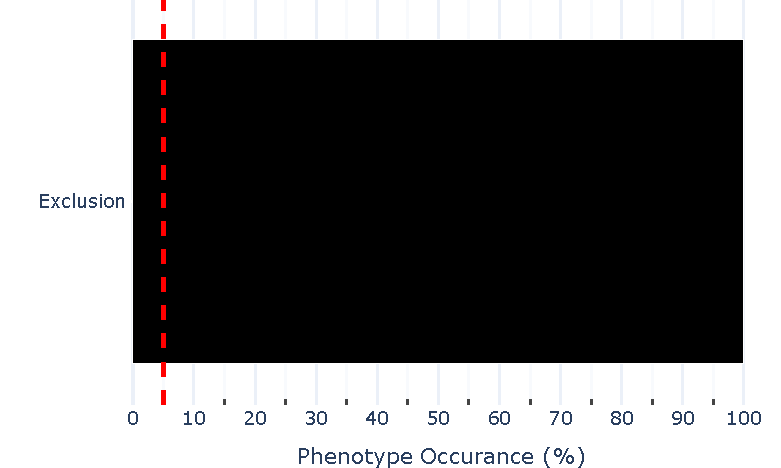
\includegraphics[width=1\linewidth]{09. Chapter 4/Figs/01. pIB/03. IFIT2/03. IFIT2B/01. bar_i2b_293t.pdf} 
    \end{subfigure}
    \begin{subfigure}{0.495\textwidth}
        \caption{}
        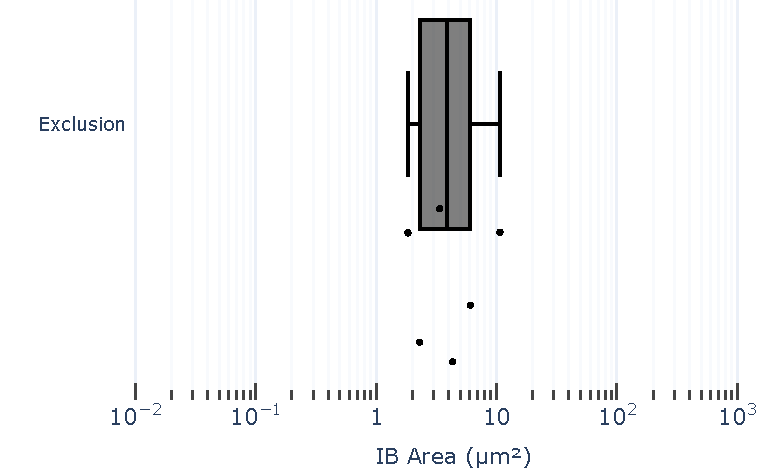
\includegraphics[width=1\linewidth]{09. Chapter 4/Figs/01. pIB/03. IFIT2/03. IFIT2B/02. box_i2b_293t.pdf}
    \end{subfigure}
    \caption[Observed Phenotypes of Endogenous Human IFIT2 in the Context of hRSV Pseudo Inclusion Bodies in 293T Cell Line, as Detected by IFIT2(B) Antibody.]{\textbf{Observed Phenotypes of Endogenous Human IFIT2 in the Context of hRSV Pseudo Inclusion Bodies in 293T Cell Line, as Detected by IFIT2(B) Antibody.} 293T cells were transfected with hRSV N and P containing plasmids using TransIT-X2 and were fixed after 24 hours. Cells were labelled with anti-RSV N and anti-IFIT2(B) antibodies and imaged on a confocal microscope. Panel (a) shows the percentual proportions of observed phenotypes between hRSV pseudo inclusion bodies and human IFIT2 (6 observations), with the red dotted line denoting the 5\% threshold, marking phenotypes considered relevant above this limit. Panel (b) shows the IB area in \(\mu \mbox{m}^2\) per observed relevant phenotype.}
    \label{fig:Observed Phenotypes of Endogenous Human IFIT2 in the Context of hRSV Pseudo Inclusion Bodies in 293T Cell Line, as Detected by IFIT2(B) Antibody}
\end{figure}

\begin{figure}
    \centering
    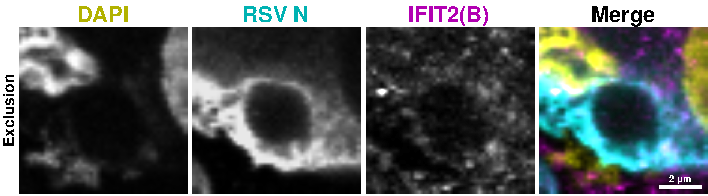
\includegraphics[width=1\linewidth]{09. Chapter 4/Figs/01. pIB/03. IFIT2/03. IFIT2B/03. i2b-293t-hnhp.pdf} 
    \caption[Representative Images of Observed Phenotypes of Endogenous Human IFIT2 in the Context of hRSV Pseudo Inclusion Bodies in 293T Cell Line, as Detected by IFIT2(B) Antibody.]{\textbf{Representative Images of Observed Phenotypes of Endogenous Human IFIT2 in the Context of hRSV Pseudo Inclusion Bodies in 293T Cell Line, as Detected by IFIT2(B) Antibody.} 293T cells were transfected with hRSV N and P containing plasmids using TransIT-X2 and were fixed after 24 hours. Cellular nuclei were stained with DAPI (yellow), and cells were double-labelled with anti-RSV N (cyan) and anti-IFIT2(B) (magenta) antibodies. This figure showcases representative examples of relevant phenotypes in the interaction between human IFIT2 and hRSV pseudo-inclusion bodies. These phenotypes are presented in descending order based on their percentage proportions. The scale bar indicates 2 \(\mu \mbox{m}\).}
    \label{fig:Representative Images of Observed Phenotypes of Endogenous Human IFIT2 in the Context of hRSV Pseudo Inclusion Bodies in 293T Cell Line, as Detected by IFIT2(B) Antibody}
\end{figure}

Next we focused on the assesment of IFIT2 interaction with hRSV pIBs as detected by the IFIT2(B) antibody. Initialy we assessed the human IFIT2 interaction to hRSV pIBs, aqured from HEK293T cell line. We have however obtained only 6 observations, all of which showed exclusion phenotype (Figure \ref{fig:Observed Phenotypes of Endogenous Human IFIT2 in the Context of hRSV Pseudo Inclusion Bodies in 293T Cell Line, as Detected by IFIT2(B) Antibody}, panel a). The measured area of these hRSV pIBs is showin in Figure \ref{fig:Observed Phenotypes of Endogenous Human IFIT2 in the Context of hRSV Pseudo Inclusion Bodies in 293T Cell Line, as Detected by IFIT2(B) Antibody}, panel b. The representative image of this phenotype is shown in Figure \ref{fig:Representative Images of Observed Phenotypes of Endogenous Human IFIT2 in the Context of hRSV Pseudo Inclusion Bodies in 293T Cell Line, as Detected by IFIT2(B) Antibody}. Although we only observed 6 pIBs, these encompasses the range where the majority of the total observed hRSV pIBs sizes were situated i.e. they ranged from sub 2 \(\mu \mbox{m}^2\) to supra 10 \(\mu \mbox{m}^2\), with the typical value of 4 \(\mu \mbox{m}^2\).

\begin{figure}
    \begin{subfigure}{0.495\textwidth}
        \caption{}
        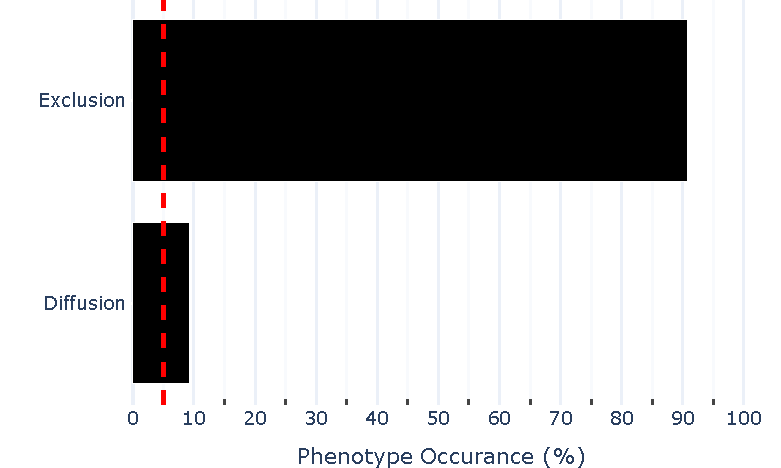
\includegraphics[width=1\linewidth]{09. Chapter 4/Figs/01. pIB/03. IFIT2/03. IFIT2B/04. bar_i2b_vero_hnhp.pdf} 
    \end{subfigure}
    \begin{subfigure}{0.495\textwidth}
        \caption{}
        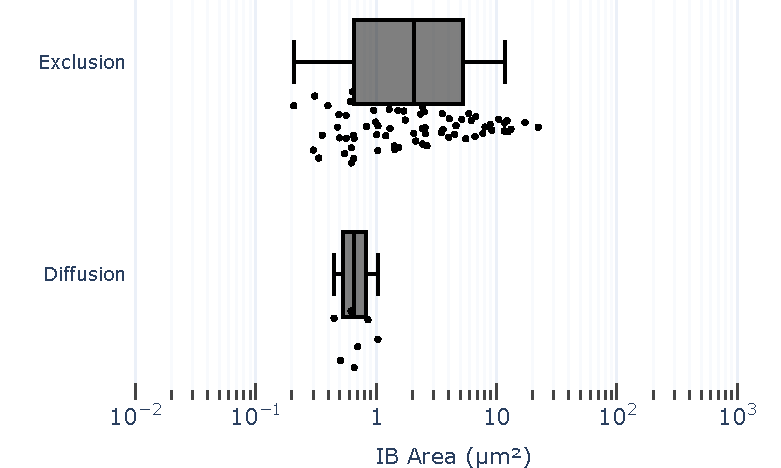
\includegraphics[width=1\linewidth]{09. Chapter 4/Figs/01. pIB/03. IFIT2/03. IFIT2B/05. box_i2b_vero_hnhp.pdf}
    \end{subfigure}
    \caption[Observed Phenotypes of Endogenous Monkey IFIT2 in the Context of hRSV Pseudo Inclusion Bodies in Vero Cell Line, as Detected by IFIT2(B) Antibody.]{\textbf{Observed Phenotypes of Endogenous Monkey IFIT2 in the Context of hRSV Pseudo Inclusion Bodies in Vero Cell Line, as Detected by IFIT2(B) Antibody.} Vero cells were transfected with hRSV N and P containing plasmids using TransIT-X2 and were fixed after 24 hours. Cells were labelled with anti-RSV N and anti-IFIT2(B) antibodies and imaged on a confocal microscope. Panel (a) shows the percentual proportions of observed phenotypes between hRSV pseudo inclusion bodies and monkey IFIT2 (76 observations), with the red dotted line denoting the 5\% threshold, marking phenotypes considered relevant above this limit. Panel (b) shows the IB area in \(\mu \mbox{m}^2\) per observed relevant phenotype.}
    \label{fig:Observed Phenotypes of Endogenous Monkey IFIT2 in the Context of hRSV Pseudo Inclusion Bodies in Vero Cell Line, as Detected by IFIT2(B) Antibody}
\end{figure}

\begin{figure}
    \centering
    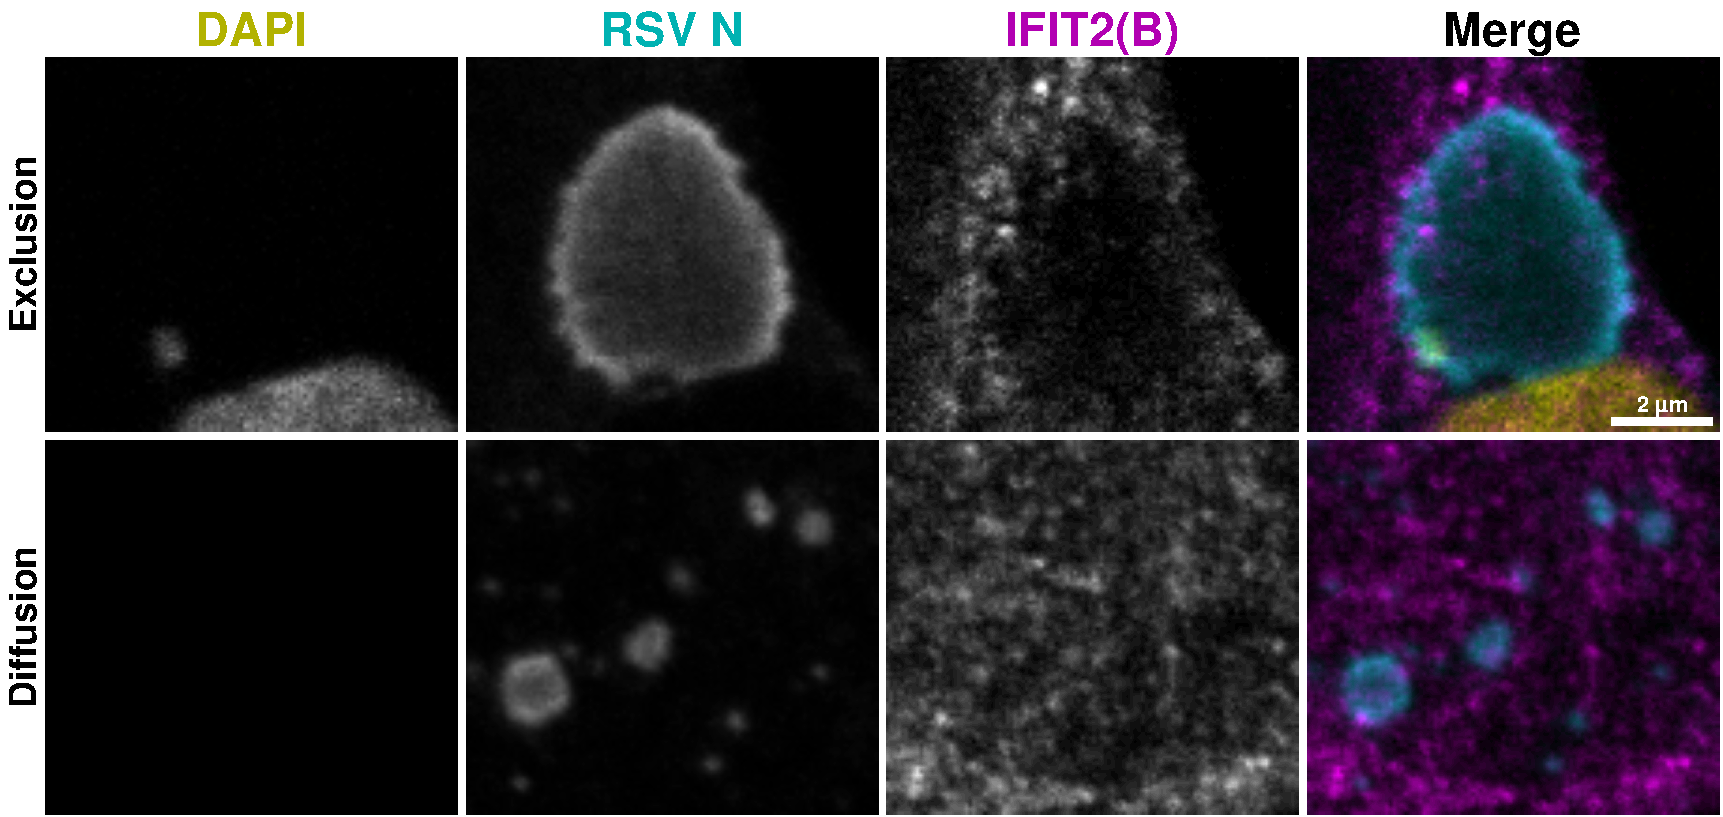
\includegraphics[width=1\linewidth]{09. Chapter 4/Figs/01. pIB/03. IFIT2/03. IFIT2B/06. i2b-vero-hnhp.pdf} 
    \caption[Representative Images of Observed Phenotypes of Endogenous Monkey IFIT2 in the Context of hRSV Pseudo Inclusion Bodies in Vero Cell Line, as Detected by IFIT2(B) Antibody.]{\textbf{Representative Images of Observed Phenotypes of Endogenous Monkey IFIT2 in the Context of hRSV Pseudo Inclusion Bodies in Vero Cell Line, as Detected by IFIT2(B) Antibody.} Vero cells were transfected with hRSV N and P containing plasmids using TransIT-X2 and were fixed after 24 hours. Cellular nuclei were stained with DAPI (yellow), and cells were double-labelled with anti-RSV N (cyan) and anti-IFIT2(B) (magenta) antibodies. This figure showcases representative examples of relevant phenotypes in the interaction between monkey IFIT2 and hRSV pseudo-inclusion bodies. These phenotypes are presented in descending order based on their percentage proportions. The scale bar indicates 2 \(\mu \mbox{m}\).}
    \label{fig:Representative Images of Observed Phenotypes of Endogenous Monkey IFIT2 in the Context of hRSV Pseudo Inclusion Bodies in Vero Cell Line, as Detected by IFIT2(B) Antibody}
\end{figure}

Finally we have assayed the endogenous monkey IFIT2 interactions with hRSV pIBs, as detected by the IFIT2(B) antibody. The observed interaction phenotypes, their respectife frequencies of occurance along with the pIB sizes denoted per observed phenotype are shown in Figure \ref{fig:Observed Phenotypes of Endogenous Monkey IFIT2 in the Context of hRSV Pseudo Inclusion Bodies in Vero Cell Line, as Detected by IFIT2(B) Antibody}. The representative images of these interactions are shown in Figure \ref{fig:Representative Images of Observed Phenotypes of Endogenous Monkey IFIT2 in the Context of hRSV Pseudo Inclusion Bodies in Vero Cell Line, as Detected by IFIT2(B) Antibody}. Within the 76 observations we have observed two phenotypes i.e. exclusion and diffusion. The former was the most prevalent and appeared in 91\% of observations, while the latter occured in 9\% of cases. The exclusion phenotype in a wide range of pIB sizes, which are quite representative of the aggregate distribution of all pIB sizes detected in the Vero cell line. In more detail, they ranged from 0.2 \(\mu \mbox{m}^2\) to 21 \(\mu \mbox{m}^2\), with the typical size of 2 \(\mu \mbox{m}^2\). The  diffusion phenotype, on the other hand, happened predominantly in smaller pIBs, ranging from 0.43 \(\mu \mbox{m}^2\) to 1 \(\mu \mbox{m}^2\), with the median size of 0.63 \(\mu \mbox{m}^2\).

Overall we have observed results of IFIT2 intraction with RSV pIBs which were very consistent to what was observed with endogenous human and bovine IFIT2 during RSV infection in Section \ref{subsec:Endogenous IFIT Interaction with RSV Inclusion Bodies}. IFIT2(B) deteted endogenous human and monkey to be excluded from hRSV pIBs, with the exception of moneky IFIT2 where it also observed diffusion to occur in 9\% of all cases. IFIT2(A) antibody on the other hand detected IFIT2 to form intra-pIB solely regardless of the host species or the species of the virus, from which the pIBs originated. This is in contrast to what we observed during infection, where both human and bovine IFIT2, as detected byb the IFIT2(A) antobody, was observed to form intra-IB inclusions in smaller IBs and to colocalise with the IB edge while being excluded from the IB interior in larger IBs. Regardless, we can still see a stark discintion between observed IFIT2 using the two antibodies while we lack the understanding of what differentiate the two hypothetised IFIT2 popoulations. Clearly the current approach is not sufficient to uncover the nature of the differences observed by these two antibodies. By detecting a distinct epitope, such as FLAG tag, we would have ncreased confidence into detecting the whole IFIT2 population. 

To do this we utilised the human IFIT2-FLAG containing plasmid, which was provided to us by the Viral Gene Expressioin group from the Pirbright Institute and by bovine IFIT2-FLAG contang plasmid, which was prepared as described in Section \ref{sec:DNA Work} and Section \ref{subsec:Overexpressed IFIT1, IFIT3, and IFIT5 During RSV Infection}. We decided to initially assess these with the context of human and bovine RSV pseudo inclusion bodies, as these yieled more defined interaction phenotypes as detected by the IFIT2(A) and IFIT2(B) antibodies. We also decided for this approach as transfection of three plasmids (i.e. N, P, and IFIT2-FLAG containing plasmids) has higher efficiency than conducting co-infection/transfection. After overexpressing the FLAG-tagged IFIT2 this would allow us to not only probe the FLAG tag to obtain the ground truth about the IFIT2 subcellular localisation with regards to RSV pIBs, it would also allow us to probe with the IFIT2(A) and IFIT2(B) antibodies to probe if their differential IFIT2 detection remains unchanged.

\begin{figure}
    \begin{subfigure}{0.495\textwidth}
        \caption{}
        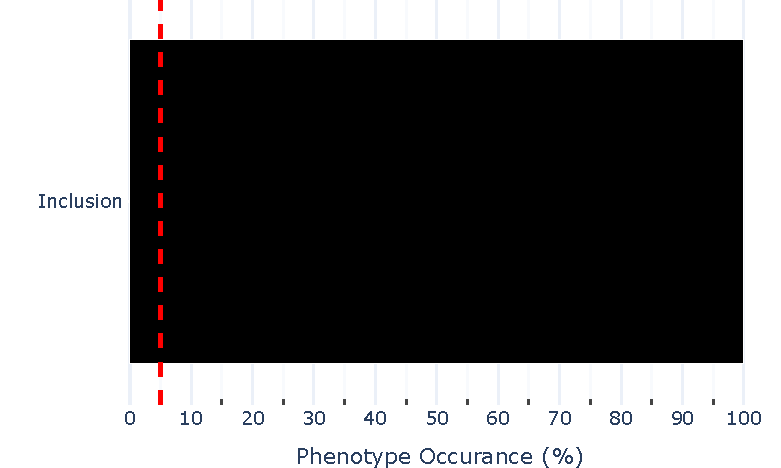
\includegraphics[width=1\linewidth]{09. Chapter 4/Figs/01. pIB/03. IFIT2/04. IFIT2-FLAG/01. IFIT2A/01. bar_i2a_hnhp.pdf} 
    \end{subfigure}
    \begin{subfigure}{0.495\textwidth}
        \caption{}
        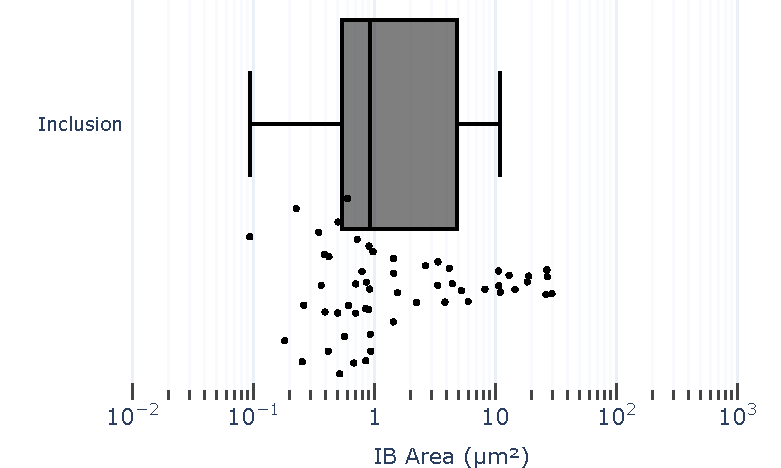
\includegraphics[width=1\linewidth]{09. Chapter 4/Figs/01. pIB/03. IFIT2/04. IFIT2-FLAG/01. IFIT2A/02. box_i2a_hnhp.pdf}
    \end{subfigure}
    \caption[Observed Phenotypes of Exogenous Human IFIT2 in the Context of hRSV Pseudo Inclusion Bodies in Vero Cell Line, as Detected by IFIT2(A) Antibody.]{\textbf{Observed Phenotypes of Exogenous Human IFIT2 in the Context of hRSV Pseudo Inclusion Bodies in Vero Cell Line, as Detected by IFIT2(A) Antibody.} Vero cells were transfected with hRSV N and P, along with human IFIT2-FLAG containing plasmids using TransIT-X2 and were fixed after 24 hours. Cells were labelled with anti-RSV N and anti-IFIT2(A) antibodies and imaged on a confocal microscope. Panel (a) shows the percentual proportions of observed phenotypes between hRSV pseudo inclusion bodies and exogenous human IFIT2 (56 observations), with the red dotted line denoting the 5\% threshold, marking phenotypes considered relevant above this limit. Panel (b) shows the IB area in \(\mu \mbox{m}^2\) per observed relevant phenotype.}
    \label{fig:Observed Phenotypes of Exogenous Human IFIT2 in the Context of hRSV Pseudo Inclusion Bodies in Vero Cell Line, as Detected by IFIT2(A) Antibody}
\end{figure}

\begin{figure}
    \centering
    \includegraphics[width=1\linewidth]{09. Chapter 4/Figs/01. pIB/03. IFIT2/04. IFIT2-FLAG/01. IFIT2A/03. i2a-hi2f-hnhp.pdf}
    \caption[Representative Images of Observed Phenotypes of Exogenous Human IFIT2 in the Context of hRSV Pseudo Inclusion Bodies in Vero Cell Line, as Detected by IFIT2(A) Antibody.]{\textbf{Representative Images of Observed Phenotypes of Exogenous Human IFIT2 in the Context of hRSV Pseudo Inclusion Bodies in Vero Cell Line, as Detected by IFIT2(A) Antibody.} Vero cells were transfected with hRSV N and P, along with human IFIT2-FLAG containing plasmids using TransIT-X2 and were fixed after 24 hours. Cellular nuclei were stained with DAPI (yellow), and cells were double-labelled with anti-RSV N (cyan) and anti-IFIT2(A) (magenta) antibodies. This figure showcases representative examples of relevant phenotypes in the interaction between exogenous human IFIT2 and hRSV pseudo-inclusion bodies. These phenotypes are presented in descending order based on their percentage proportions. The scale bar indicates 2 \(\mu \mbox{m}\).}
    \label{fig:Representative Images of Observed Phenotypes of Exogenous Human IFIT2 in the Context of hRSV Pseudo Inclusion Bodies in Vero Cell Line, as Detected by IFIT2(A) Antibody}
\end{figure}

Firstly we expressed the human IFIT2-FLAG in the context of hRSV pseudo-IBs in the Vero cell line, and detected the IFIT2 usiong the IFIT2(A) antibody. We determined which cells were sucessfuly transfected with hIFIT2-FLAG depending on the increased IFIT2 signal compared to the surrounding cells (data not shown). We have observed 56 observations, which all displayed the inclusion phenotype (Figure \ref{fig:Observed Phenotypes of Exogenous Human IFIT2 in the Context of hRSV Pseudo Inclusion Bodies in Vero Cell Line, as Detected by IFIT2(A) Antibody}, panel a). The observed pIBs ranged in size from 0.09 \(\mu \mbox{m}^2\) to 29 \(\mu \mbox{m}^2\), with the median value of \(\mu \mbox{m}^2\) (Figure \ref{fig:Observed Phenotypes of Exogenous Human IFIT2 in the Context of hRSV Pseudo Inclusion Bodies in Vero Cell Line, as Detected by IFIT2(A) Antibody}, panel b). We have observed IFIT2 to form inclusions within nuclear pIBs as well, a phenomenon which will be decribed more bellow. The representative images of cellular and nuclear inclusions are shown in Figure \ref{fig:Representative Images of Observed Phenotypes of Exogenous Human IFIT2 in the Context of hRSV Pseudo Inclusion Bodies in Vero Cell Line, as Detected by IFIT2(A) Antibody}.

\begin{figure}
    \begin{subfigure}{0.495\textwidth}
        \caption{}
        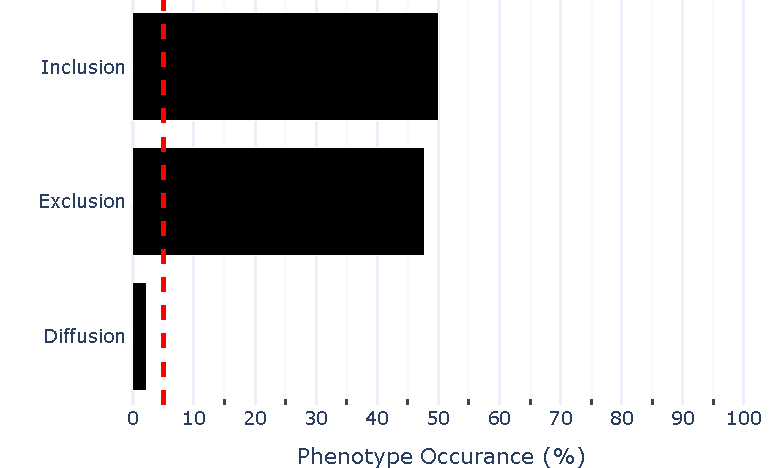
\includegraphics[width=1\linewidth]{09. Chapter 4/Figs/01. pIB/03. IFIT2/04. IFIT2-FLAG/02. IFIT2B/01. bar_i2b_hnhp.pdf}
    \end{subfigure}
    \begin{subfigure}{0.495\textwidth}
        \caption{}
        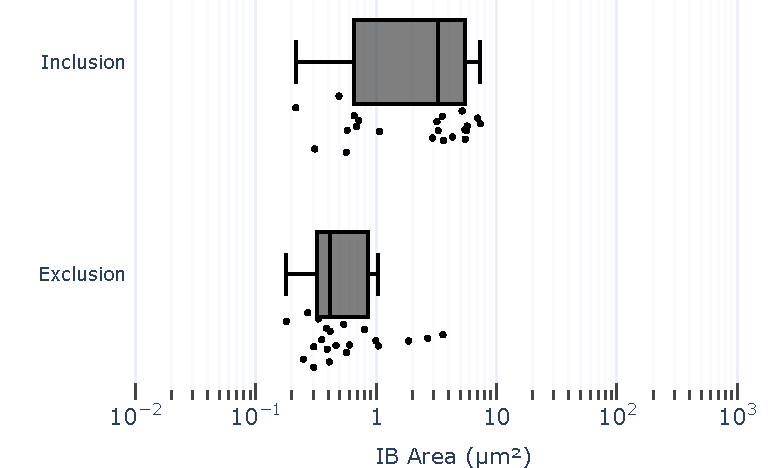
\includegraphics[width=1\linewidth]{09. Chapter 4/Figs/01. pIB/03. IFIT2/04. IFIT2-FLAG/02. IFIT2B/02. box_i2a_hnhp.pdf}
    \end{subfigure}
    \caption[Observed Phenotypes of Exogenous Human IFIT2 in the Context of hRSV Pseudo Inclusion Bodies in Vero Cell Line, as Detected by IFIT2(B) Antibody.]{\textbf{Observed Phenotypes of Exogenous Human IFIT2 in the Context of hRSV Pseudo Inclusion Bodies in Vero Cell Line, as Detected by IFIT2(B) Antibody.} Vero cells were transfected with hRSV N and P, along with human IFIT2-FLAG containing plasmids using TransIT-X2 and were fixed after 24 hours. Cells were labelled with anti-RSV N and anti-IFIT2(B) antibodies and imaged on a confocal microscope. Panel (a) shows the percentual proportions of observed phenotypes between hRSV pseudo inclusion bodies and exogenous human IFIT2 (44 observations), with the red dotted line denoting the 5\% threshold, marking phenotypes considered relevant above this limit. Panel (b) shows the IB area in \(\mu \mbox{m}^2\) per observed relevant phenotype.}
    \label{fig:Observed Phenotypes of Exogenous Human IFIT2 in the Context of hRSV Pseudo Inclusion Bodies in Vero Cell Line, as Detected by IFIT2(B) Antibody}
\end{figure}

\begin{figure}
    \centering
    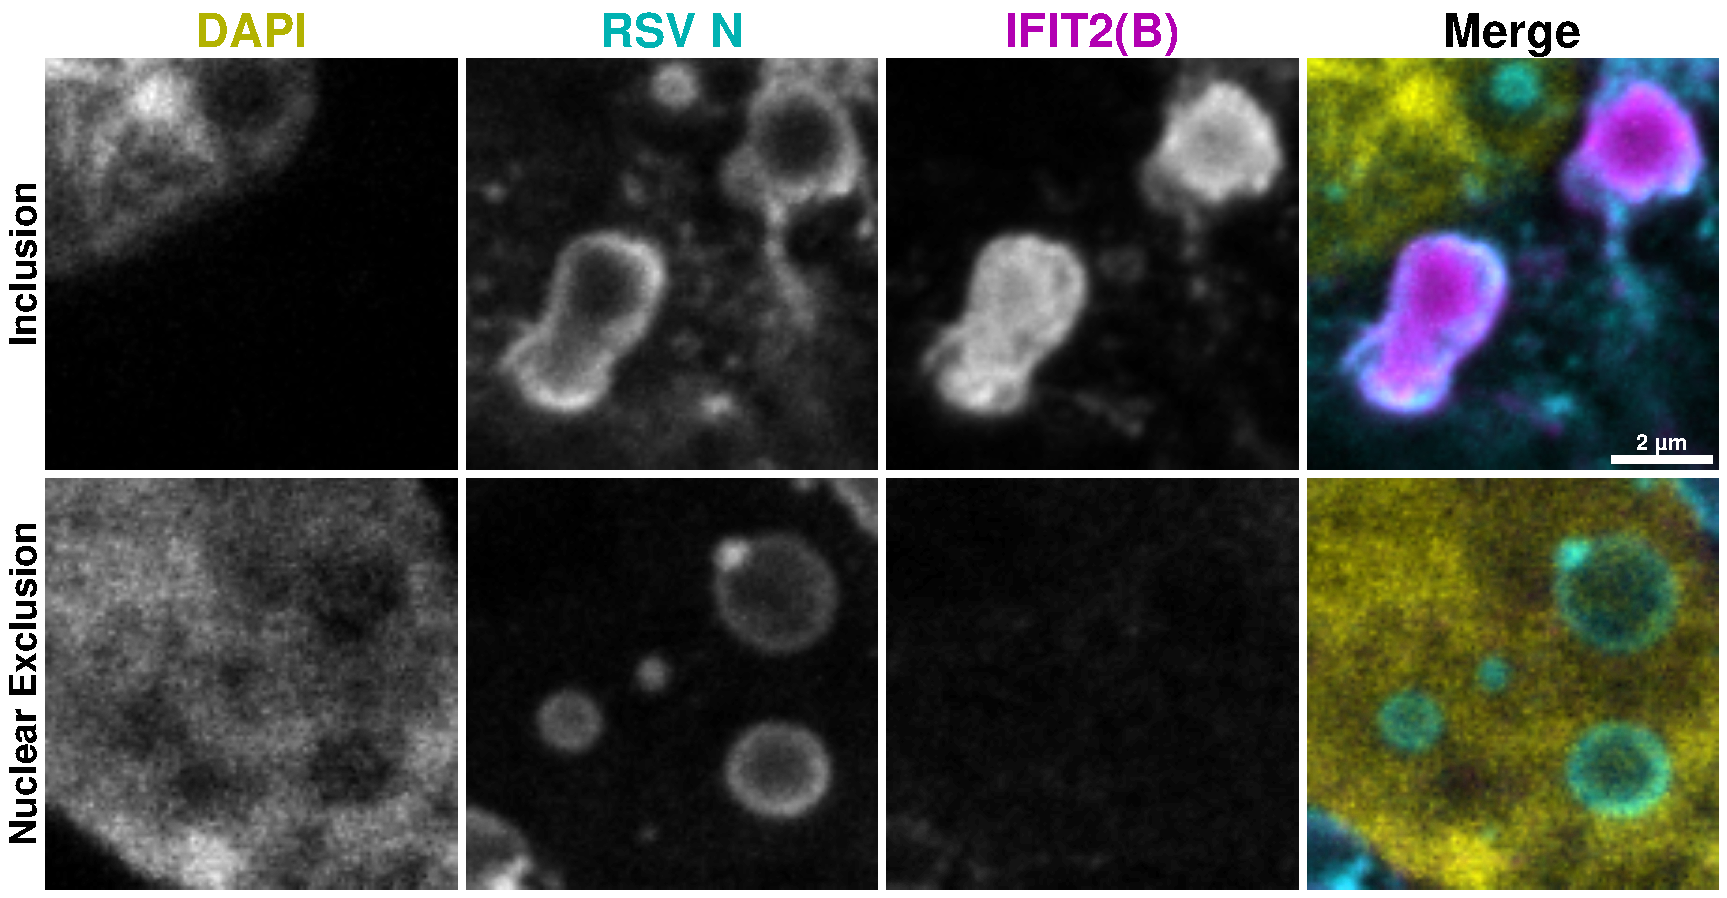
\includegraphics[width=1\linewidth]{09. Chapter 4/Figs/01. pIB/03. IFIT2/04. IFIT2-FLAG/02. IFIT2B/03. i2b-hi2f-hnhp.pdf}
    \caption[Representative Images of Observed Phenotypes of Exogenous Human IFIT2 in the Context of hRSV Pseudo Inclusion Bodies in Vero Cell Line, as Detected by IFIT2(B) Antibody.]{\textbf{Representative Images of Observed Phenotypes of Exogenous Human IFIT2 in the Context of hRSV Pseudo Inclusion Bodies in Vero Cell Line, as Detected by IFIT2(B) Antibody.} Vero cells were transfected with hRSV N and P, along with human IFIT2-FLAG containing plasmids using TransIT-X2 and were fixed after 24 hours. Cellular nuclei were stained with DAPI (yellow), and cells were double-labelled with anti-RSV N (cyan) and anti-IFIT2(B) (magenta) antibodies. This figure showcases representative examples of relevant phenotypes in the interaction between exogenous human IFIT2 and hRSV pseudo-inclusion bodies. These phenotypes are presented in descending order based on their percentage proportions. The scale bar indicates 2 \(\mu \mbox{m}\).}
    \label{fig:Representative Images of Observed Phenotypes of Exogenous Human IFIT2 in the Context of hRSV Pseudo Inclusion Bodies in Vero Cell Line, as Detected by IFIT2(B) Antibody}
\end{figure}

Next we replicated the previous expreiment using the IFIT2(B) antibody for exogenous human IFIT2-FLAG detection. We have obtained 44 observations of IFIT2-pIB interactions. The observed interaction, their frequencies of occurance, along with the pIB sizes associated with the phenotypes that occured with more than 5\% frequency are shown in the Figure \ref{fig:Observed Phenotypes of Exogenous Human IFIT2 in the Context of hRSV Pseudo Inclusion Bodies in Vero Cell Line, as Detected by IFIT2(B) Antibody}. The representative images of the latter are shown in Figure \ref{fig:Representative Images of Observed Phenotypes of Exogenous Human IFIT2 in the Context of hRSV Pseudo Inclusion Bodies in Vero Cell Line, as Detected by IFIT2(B) Antibody}. Suprisingly, the most common interaction phenotype was inclusion which occured in half of the observations. This was closely followed by exclusion phenotype, which occured in 47\% of cases. Lastly, wqe have observed 3\% of observations to conform to the diffusion phenotype. While the inclusion phenotype occured in pIBs of a broad size range, from 0.21 \(\mu \mbox{m}^2\) to 7.2 \(\mu \mbox{m}^2\), with the median value of 3.2 \(\mu \mbox{m}^2\), the exclusion phenotype occured predominantly in smaller pIBs, which ranged from sub 0.2 \(\mu \mbox{m}^2\) to 3.5 \(\mu \mbox{m}^2\), with the median value of 0.4 \(\mu \mbox{m}^2\). We have observed the exclusion-associated pIBs to be located withing the boundry of a nucleus. Taking all of thius together, both IFIT2(A) and IFIT2(B) antibodies detect exogenously expressed hIFIT2-FLAG to form intra-pIB inclusios. We still observe a discrepancy between the antibodies i.e. IFIT2(A) detected IFIT2 to be forming inclusions within nuclear pIBs, while IFIT2(B) antibody observed IFIT2 to be excluded from these. Both antibodies did not detect IFIT2 withiin the nucleoplasm. Due to the persistent differential staining of the two antibodies it is imperative to probe the exogenous IFIT2 using anti-FLAG antibody.

\begin{figure}
    \begin{subfigure}{0.495\textwidth}
        \caption{}
        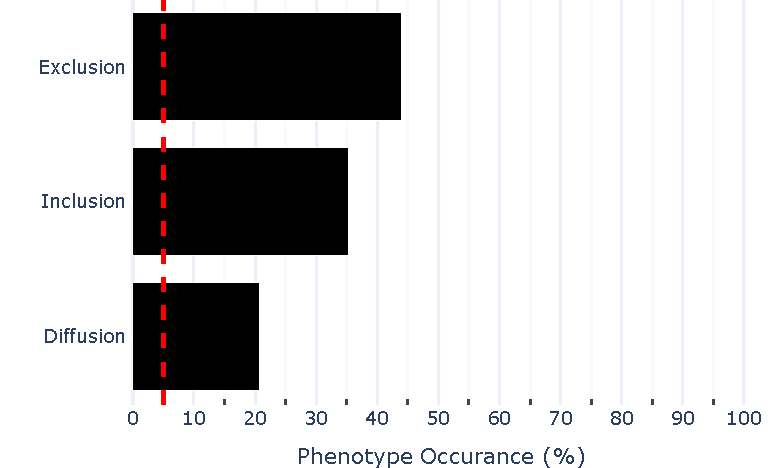
\includegraphics[width=1\linewidth]{09. Chapter 4/Figs/01. pIB/03. IFIT2/04. IFIT2-FLAG/03. FLAG/01. bar_hi2f_hnhp.pdf}
    \end{subfigure}
    \begin{subfigure}{0.495\textwidth}
        \caption{}
        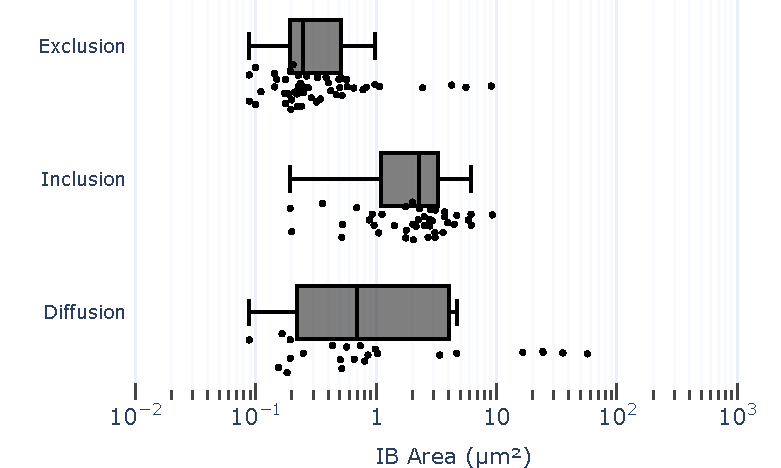
\includegraphics[width=1\linewidth]{09. Chapter 4/Figs/01. pIB/03. IFIT2/04. IFIT2-FLAG/03. FLAG/02. box_hi2f_hnhp.pdf}
    \end{subfigure}
    \caption[Observed Phenotypes of Exogenous Human IFIT2 in the Context of hRSV Pseudo Inclusion Bodies in Vero Cell Line, as Detected by FLAG Antibody.]{\textbf{Observed Phenotypes of Exogenous Human IFIT2 in the Context of hRSV Pseudo Inclusion Bodies in Vero Cell Line, as Detected by FLAG Antibody.} Vero cells were transfected with hRSV N and P, along with human IFIT2-FLAG containing plasmids using TransIT-X2 and were fixed after 24 hours. Cells were labelled with anti-RSV N and anti-FLAG antibodies and imaged on a confocal microscope. Panel (a) shows the percentual proportions of observed phenotypes between hRSV pseudo inclusion bodies and exogenous human IFIT2 (116 observations), with the red dotted line denoting the 5\% threshold, marking phenotypes considered relevant above this limit. Panel (b) shows the IB area in \(\mu \mbox{m}^2\) per observed relevant phenotype.}
    \label{fig:Observed Phenotypes of Exogenous Human IFIT2 in the Context of hRSV Pseudo Inclusion Bodies in Vero Cell Line, as Detected by FLAG Antibody}
\end{figure}

\begin{figure}
    \centering
    \includegraphics[width=1\linewidth]{09. Chapter 4/Figs/01. pIB/03. IFIT2/04. IFIT2-FLAG/03. FLAG/03. hi2f-hnhp.pdf}
    \caption[Representative Images of Observed Phenotypes of Exogenous Human IFIT2 in the Context of hRSV Pseudo Inclusion Bodies in Vero Cell Line, as Detected by FLAG Antibody.]{\textbf{Representative Images of Observed Phenotypes of Exogenous Human IFIT2 in the Context of hRSV Pseudo Inclusion Bodies in Vero Cell Line, as Detected by FLAG Antibody.} Vero cells were transfected with hRSV N and P, along with human IFIT2-FLAG containing plasmids using TransIT-X2 and were fixed after 24 hours. Cellular nuclei were stained with DAPI (yellow), and cells were double-labelled with anti-RSV N (cyan) and anti-FLAG (magenta) antibodies. This figure showcases representative examples of relevant phenotypes in the interaction between exogenous human IFIT2 and hRSV pseudo-inclusion bodies. These phenotypes are presented in descending order based on their percentage proportions. The scale bar indicates 2 \(\mu \mbox{m}\).}
    \label{fig:Representative Images of Observed Phenotypes of Exogenous Human IFIT2 in the Context of hRSV Pseudo Inclusion Bodies in Vero Cell Line, as Detected by FLAG Antibody}
\end{figure}

Using the anti-FLAG antibody we have probed the true localisation of exogenously expressed human IFIT2-FLAG and its interaction with hRSV pIBs. The frequenbcies of occureances of the observed interaction phenotypes, based on 116 observations, along with the measured pIB sizes, based on the phenotype associations are shown in Figure \ref{fig:Observed Phenotypes of Exogenous Human IFIT2 in the Context of hRSV Pseudo Inclusion Bodies in Vero Cell Line, as Detected by FLAG Antibody}. The representative images of these phenotyeps are shown in Figure \ref{fig:Representative Images of Observed Phenotypes of Exogenous Human IFIT2 in the Context of hRSV Pseudo Inclusion Bodies in Vero Cell Line, as Detected by FLAG Antibody}. The most common phenotype was exclusio from the pIB structures, which occured in 49\% of observations. This was followed by intra-pIB incusions, which occured at the frequency of 35\%. Lastly, we have detected IFIT2 to be diffused equally throught the cytoplasm and the pIB structure in 21\% of observations. The exclusion appeared in predominantly smaller sub 1 \(\mu \mbox{m}^2\) pIBs, although we have observed 4 pIBs which were associated with this phenotype and were larger then this. In more detail, exclusion-associated pIBs ranged from 0.09 \(\mu \mbox{m}^2\) to 9 \(\mu \mbox{m}^2\), with the typical value of 0.23 \(\mu \mbox{m}^2\). These pIBs were also located within the boundry of nucleus. The inclusion-associated pIBs ranged from 0.2 \(\mu \mbox{m}^2\) to 9 \(\mu \mbox{m}^2\), with the median value of 2.1 \(\mu \mbox{m}^2\). Latrly, while the diffusion phenotype occured with predominantly small, sub 1 \(\mu \mbox{m}^2\) pIBs, we haveobserved 6 outliers that were each progresively larger. In general the diffusion-associated pIBs ranged from 0.09 \(\mu \mbox{m}^2\) to 55 \(\mu \mbox{m}^2\), with the median value of just 0.7 \(\mu \mbox{m}^2\). 

These data are conbsistent with that was oibserved in overexpressed hIFIT2-FLAG as detected by the IFIT2(B) antibody, which suggest this antibody more realisticvaly portray the IFIT2 population. It is intreeuging that ecopic expression of IFIT2 suddenly enable IFIT2(B) antibody to detect IFIT2 froming intra pIB iunclusions. This obsevation is difficult to explain, but we suspect it can be as a result exogenous IFIT2-FLAG losing some of its interaction partners, potentialy due to the C-terninal FLAG tag. This data also indicates that our previous assumpton was correct meaning the real interaction of IFIT2 with regarsd to both IB and pIB interaction is both excluson and strong interacton phenotypes (inclusion or colocalisation associated with exclusion), which occur approximately in the same frequency. Another intreeuging fast is that while both IFIT2(B) and FLAG antobodies did not detect IFIT2 interaction with the nucleus associated pIBs, the IFIT2(A) antibody was able to detect inclusions. This could be possibly explained by IFIT2(A) off tasrget effects, or by some mechanism which we do not comprehend yet.

\begin{figure}
    \begin{subfigure}{0.495\textwidth}
        \caption{}
        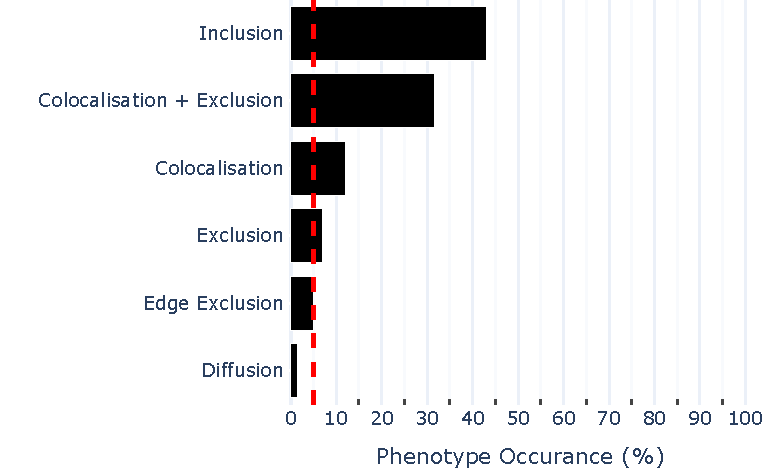
\includegraphics[width=1\linewidth]{09. Chapter 4/Figs/01. pIB/03. IFIT2/04. IFIT2-FLAG/03. FLAG/04. bar_bi2f_hnhp.pdf} 
    \end{subfigure}
    \begin{subfigure}{0.495\textwidth}
        \caption{}
        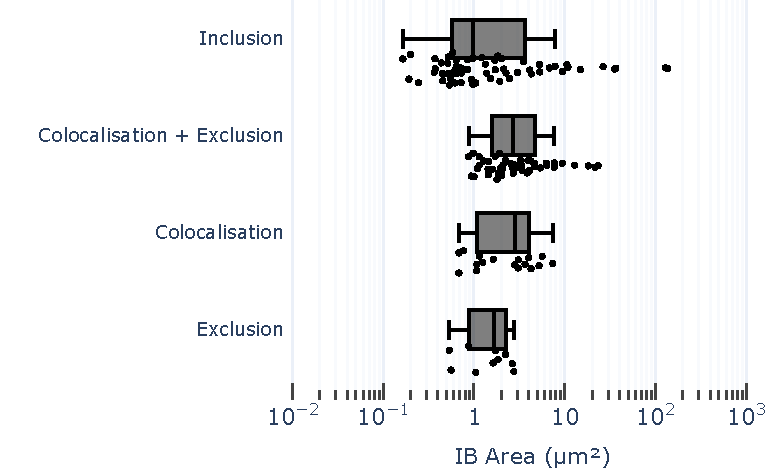
\includegraphics[width=1\linewidth]{09. Chapter 4/Figs/01. pIB/03. IFIT2/04. IFIT2-FLAG/03. FLAG/05. box_bi2f_hnhp.pdf}
    \end{subfigure}
    \caption[Observed Phenotypes of Exogenous Bovine IFIT2 in the Context of hRSV Pseudo Inclusion Bodies in Vero Cell Line, as Detected by FLAG Antibody.]{\textbf{Observed Phenotypes of Exogenous Bovine IFIT2 in the Context of hRSV Pseudo Inclusion Bodies in Vero Cell Line, as Detected by FLAG Antibody.} Vero cells were transfected with hRSV N (or N-GFP) and P, along with bovine IFIT2-FLAG containing plasmids using TransIT-X2 and were fixed after 24 hours. Cells were labelled with anti-RSV N and anti-FLAG antibodies and imaged on a confocal microscope. The N-GFP containig pIBs were visualised using the inate fuorescence of the GFP. Panel (a) shows the percentual proportions of observed phenotypes between hRSV pseudo inclusion bodies and exogenous bovine IFIT2 (142 observations), with the red dotted line denoting the 5\% threshold, marking phenotypes considered relevant above this limit. Panel (b) shows the IB area in \(\mu \mbox{m}^2\) per observed relevant phenotype.}
    \label{fig:Observed Phenotypes of Exogenous Bovine IFIT2 in the Context of hRSV Pseudo Inclusion Bodies in Vero Cell Line, as Detected by FLAG Antibody}
\end{figure}

\begin{figure}
    \centering
    \includegraphics[width=1\linewidth]{09. Chapter 4/Figs/01. pIB/03. IFIT2/04. IFIT2-FLAG/03. FLAG/06. bi2f-hnhp.pdf}
    \caption[Representative Images of Observed Phenotypes of Exogenous Bovine IFIT2 in the Context of hRSV Pseudo Inclusion Bodies in Vero Cell Line, as Detected by FLAG Antibody.]{\textbf{Representative Images of Observed Phenotypes of Exogenous Bovine IFIT2 in the Context of hRSV Pseudo Inclusion Bodies in Vero Cell Line, as Detected by FLAG Antibody.} Vero cells were transfected with hRSV N (or N-GFP) and P, along with bovine IFIT2-FLAG containing plasmids using TransIT-X2 and were fixed after 24 hours. Cellular nuclei were stained with DAPI (yellow), and cells were double-labelled with anti-RSV N (cyan) and anti-FLAG (magenta) antibodies. The N-GFP containig pIBs were visualised using the inate fuorescence of the GFP (colocalisation + exclusion phenotype). This figure showcases representative examples of relevant phenotypes in the interaction between exogenous bovine IFIT2 and hRSV pseudo-inclusion bodies. These phenotypes are presented in descending order based on their percentage proportions. The scale bar indicates 2 \(\mu \mbox{m}\).}
    \label{fig:Representative Images of Observed Phenotypes of Exogenous Bovine IFIT2 in the Context of hRSV Pseudo Inclusion Bodies in Vero Cell Line, as Detected by FLAG Antibody}
\end{figure}

We continued to investigation of IFIT2-FLAG interacton with pIB structures, now solely using the FLAG antibody. We have tried to obtain data from exogenous human IFIT2-FLAG with regards to bRSV pIBs, however, we failed to detect a single cell that would be co-transfected by all three of the required plasmids. Because of this we carried on with our nvestigation with exogenously expressed bovine IFIT2-FLAG with regards to the human and bovine RSV pseudo inclusoin bodies. Firstly we investigated overexpressed bIFIT2-FLAG and its interaction with hRSV pIBs. The pIBs were induced using the co-transfection of RSV \textit{P}-containing plasmid with either hRSV \textit{N}- or \textit{N-GFP}-containing plasmids. The GFP signal is more sensitive and reveals N being distributed through the pIB. These samples were obtained from Vero cell line and detected using anti-FALG antibody. We hvae obtanied 142 observations of bIFIT2-hRSV pIB interactions, which revealed a diverse range of interaction phenotypes. These phenotypes with their occurances frequencies, aloing with the measured sizes of pIBs per observed phenotype thart accured with more than 5\% frequency are shown in Figure \ref{fig:Observed Phenotypes of Exogenous Bovine IFIT2 in the Context of hRSV Pseudo Inclusion Bodies in Vero Cell Line, as Detected by FLAG Antibody}. The representative images of the latter are shown in Figure \ref{fig:Representative Images of Observed Phenotypes of Exogenous Bovine IFIT2 in the Context of hRSV Pseudo Inclusion Bodies in Vero Cell Line, as Detected by FLAG Antibody}. We have observed bovine IFIT2-FLAG to forim intra pIB inclusions in 46\% of all observations. This was followed by the colocalisation associated with exclusion phenotype, which appeared in 31\% of cases. It was mostly prevelant in pIBs created using the transfection of hRSV \textit{P} and \textit{N-GFP} containing plasmids. Next most prevelant phenotype was colocalisatioin, whch occured in 12\% of observations. This means that exogenous bovine IFIT2 displays strong interaction phenotypes with 89\% frequency. The resulting 11\% of observatioins were composed of exclusion (6\%), edge exclusion (4\%), and diffusion (1\%) phenotypes. The inclusion occured in pIBs that spanned the whole size spectra, from sub 0.2 \(\mu \mbox{m}^2\) to the maximum of 120 \(\mu \mbox{m}^2\), with the median value of 1 \(\mu \mbox{m}^2\). Thsi phenotype was the m,ost common out of all pIBs which had smaller area than 1 \(\mu \mbox{m}^2\), and were the only phenotype occuring in pIBs that were sub 0.5 \(\mu \mbox{m}^2\) in size. The colocalisation associated with exclusion phenotype occured in pIB that ranged 0.9 \(\mu \mbox{m}^2\) to 21 \(\mu \mbox{m}^2\) in size, with a typical value of 2.8 \(\mu \mbox{m}^2\). The same median value was observed for the colocalisation phenotype, howerer the overal distribution was shifted towards smaller size and ranged from 0.7 \(\mu \mbox{m}^2\) to 7.5 \(\mu \mbox{m}^2\). Lastly, the exclusion phenotype displayed the most compact size range i.e. from 0.53 \(\mu \mbox{m}^2\) to sub 3 \(\mu \mbox{m}^2\), with the median value of 1.7 \(\mu \mbox{m}^2\). This data suggest a size separation of observed phenotypes, where IFIT2 associated with small pIBs forms inclusions inside them, while the IFIT2 associated to the medium sized pIBs mainly confonts to colocalisaion phenotypes, either without or with associated exclusion.

\begin{figure}
    \begin{subfigure}{0.495\textwidth}
        \caption{}
        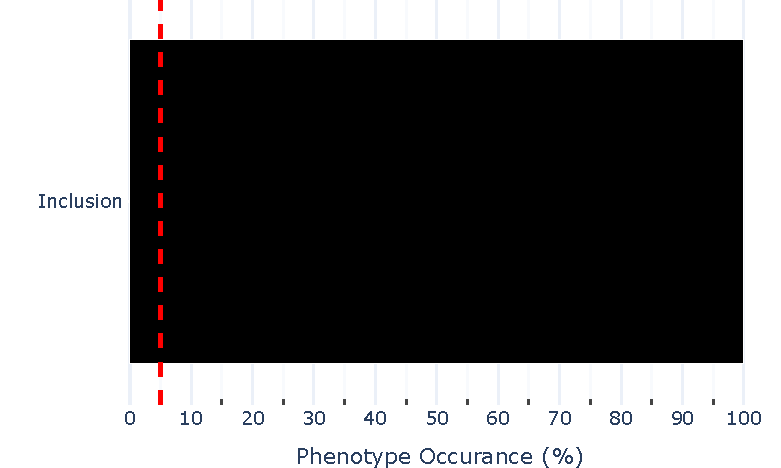
\includegraphics[width=1\linewidth]{09. Chapter 4/Figs/01. pIB/03. IFIT2/04. IFIT2-FLAG/03. FLAG/07. bar_bi2f_bnbp.pdf} 
    \end{subfigure}
    \begin{subfigure}{0.495\textwidth}
        \caption{}
        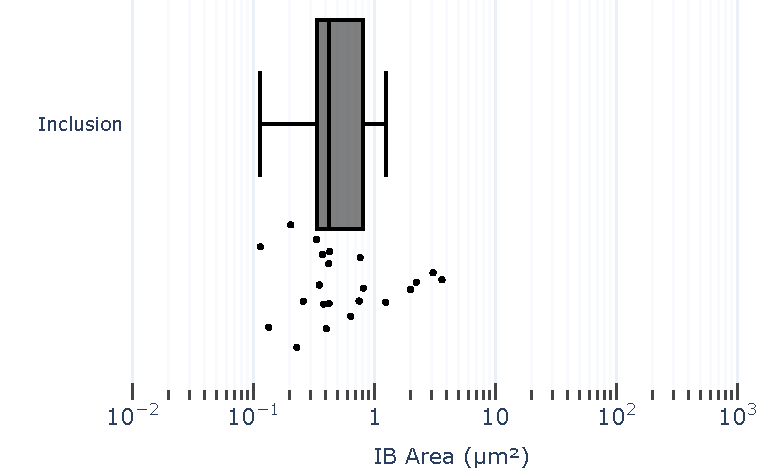
\includegraphics[width=1\linewidth]{09. Chapter 4/Figs/01. pIB/03. IFIT2/04. IFIT2-FLAG/03. FLAG/08. box_bi2f_bnbp.pdf}
    \end{subfigure}
    \caption[Observed Phenotypes of Exogenous Bovine IFIT2 in the Context of bRSV Pseudo Inclusion Bodies in Vero Cell Line, as Detected by FLAG Antibody.]{\textbf{Observed Phenotypes of Exogenous Bovine IFIT2 in the Context of bRSV Pseudo Inclusion Bodies in Vero Cell Line, as Detected by FLAG Antibody.} Vero cells were transfected with bRSV N and P, along with bovine IFIT2-FLAG containing plasmids using TransIT-X2 and were fixed after 24 hours. Cells were labelled with anti-RSV N and anti-FLAG antibodies and imaged on a confocal microscope. Panel (a) shows the percentual proportions of observed phenotypes between bRSV pseudo inclusion bodies and exogenous bovine IFIT2 (22 observations), with the red dotted line denoting the 5\% threshold, marking phenotypes considered relevant above this limit. Panel (b) shows the IB area in \(\mu \mbox{m}^2\) per observed relevant phenotype.}
    \label{fig:Observed Phenotypes of Exogenous Bovine IFIT2 in the Context of bRSV Pseudo Inclusion Bodies in Vero Cell Line, as Detected by FLAG Antibody}
\end{figure}

\begin{figure}
    \centering
    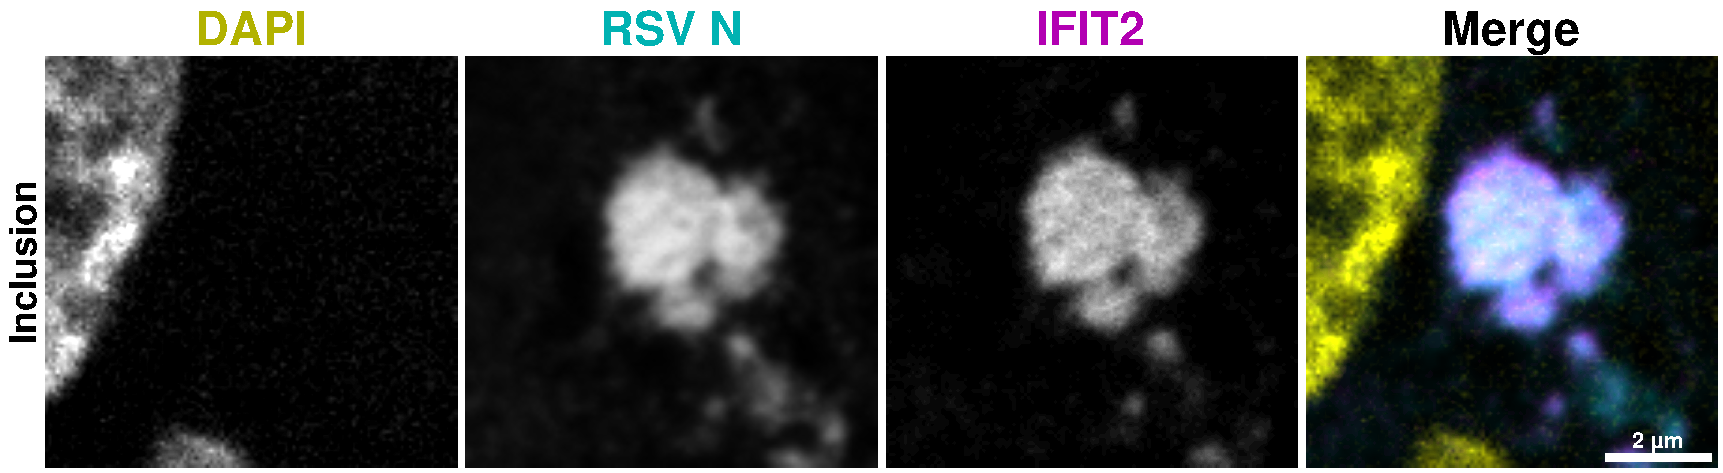
\includegraphics[width=1\linewidth]{09. Chapter 4/Figs/01. pIB/03. IFIT2/04. IFIT2-FLAG/03. FLAG/09. bi2f-bnbp.pdf}
    \caption[Representative Images of Observed Phenotypes of Exogenous Bovine IFIT2 in the Context of bRSV Pseudo Inclusion Bodies in Vero Cell Line, as Detected by FLAG Antibody.]{\textbf{Representative Images of Observed Phenotypes of Exogenous Bovine IFIT2 in the Context of bRSV Pseudo Inclusion Bodies in Vero Cell Line, as Detected by FLAG Antibody.} Vero cells were transfected with bRSV N and P, along with bovine IFIT2-FLAG containing plasmids using TransIT-X2 and were fixed after 24 hours. Cellular nuclei were stained with DAPI (yellow), and cells were double-labelled with anti-RSV N (cyan) and anti-FLAG (magenta) antibodies. This figure showcases representative examples of relevant phenotypes in the interaction between exogenous bovine IFIT2 and bRSV pseudo-inclusion bodies. These phenotypes are presented in descending order based on their percentage proportions. The scale bar indicates 2 \(\mu \mbox{m}\).}
    \label{fig:Representative Images of Observed Phenotypes of Exogenous Bovine IFIT2 in the Context of bRSV Pseudo Inclusion Bodies in Vero Cell Line, as Detected by FLAG Antibody}
\end{figure}

Lastly we investigated the phenotypic interactions of exogenously expressed bovine IFIT2-FLAG and the bRSV pIBs, as detected byb bthe anti-FLAG antibody. Due to the troubles with bRSV \textit{P} and \textit{N}-cointaing plasmid transfection we have only gathered 22 observations. All of them showed bIFT2 to form intra-pIB inclusion (Figure \ref{fig:Observed Phenotypes of Exogenous Bovine IFIT2 in the Context of bRSV Pseudo Inclusion Bodies in Vero Cell Line, as Detected by FLAG Antibody}, panel a). The representative image of this interaction is shown in Figure \ref{fig:Representative Images of Observed Phenotypes of Exogenous Bovine IFIT2 in the Context of bRSV Pseudo Inclusion Bodies in Vero Cell Line, as Detected by FLAG Antibody}. Strangely enough we have observed predomintly small pIBs in this dataset, which ranged from 0.11 \(\mu \mbox{m}^2\) to 3.5 \(\mu \mbox{m}^2\), with a median size of only 0.41 \(\mu \mbox{m}^2\) (Figure \ref{fig:Observed Phenotypes of Exogenous Bovine IFIT2 in the Context of bRSV Pseudo Inclusion Bodies in Vero Cell Line, as Detected by FLAG Antibody}, panel b). It is possible that if we would also observed larger pIBs, bIFIT2 would interact with these by colocalisaion with their boundary, as we observed with hRSV pIBs.

Taken together, we believe that probing for exogenous human and bovine IFIT2-FLAG localisation with the anti-FLAG antibody results in observation of true IFIT2 localisation, which is independent of access to IFIT2 epitopes that might be hidden while IFIT2 is interacting with its interaction partners. Using it we have uncovered that exogenously expressed human IFIT2 with regards to the hRSV pIBs, dysplayes the phenotypes that were individualy uncovered using IFIT2(A) and IFIT2(B) antibodies i.e. exclusion, incluson, and diffusion phenotypes. The exogenously expressed bovine IFIT2-FLAG on the other hand mainly dysplaed strong interacton phenotypes with regards to both human and bovine pIB. In more detail, we have observed bIFIT2 to exhibit a diverse range of phenotypic interactions with hRSV pIBs, that ranged from inclusion and colocalisation to exclusion and diffusion. 89\% of observations however conisted of inclusion, colocalisation associated with exclusion, and colocalisation phenotypes. With regards to bIFIT2 interaction with bRSV pIBs, we have observed results which were quite consistrent with what occured with hRSV pIBs. We have observed bIFIT2 to form intra-pIB iinclusion, although this dataset did not include large pIBs, and thus it is possible that if these would be present we would observe colocalisation phenotype as well. It is intreeuging to see the strriking differences in interaction phenotypes of IFIT2/pIB, which  imply the opposite spectrum of interactioni (colocalisation/inclusion vs exlusion phenotypes). Knowng from literature that IFIT2 can have its function (apoptosis) inhibited by expression of IFIT3 protein, which disrupts the action of IFIT2 homodimer by creatiion of IFIT2/IFIT3 heterodimer \cite{Mears2018BetterResponse, Stawowczyk2011TheApoptosis}, we hypothethised this interaction could be behind the observed striking differences in possible localisations. We have tried to induce human or bovine pIBs, while co-currently transfecting the IFIT2-FLAG plasmid along with human IFIT3 plasmid, which contained HA tag in its C-terminus. We have tried this many times but we never achieved sufficient IFIT3 signal in cells coexpressing RSV pseudo IBs and IFIT2.

\begin{figure}
    \begin{subfigure}{0.495\textwidth}
        \caption{}
        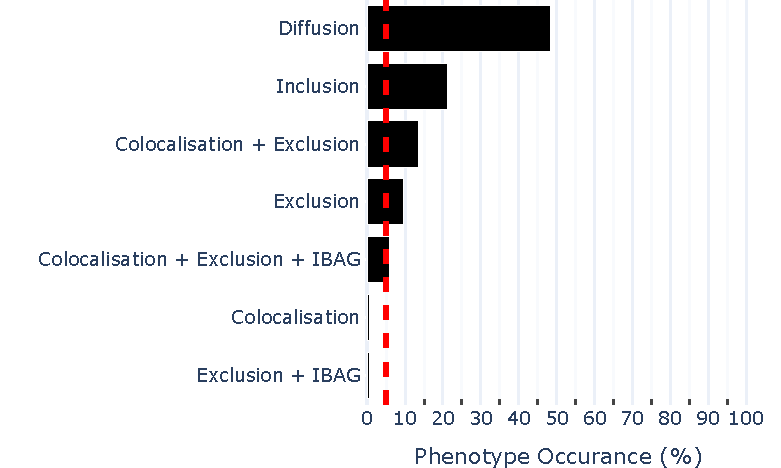
\includegraphics[width=1\linewidth]{09. Chapter 4/Figs/02. Overexpression/02. IFIT2/01. bar_hi2f_hrsv.pdf} 
    \end{subfigure}
    \begin{subfigure}{0.495\textwidth}
        \caption{}
        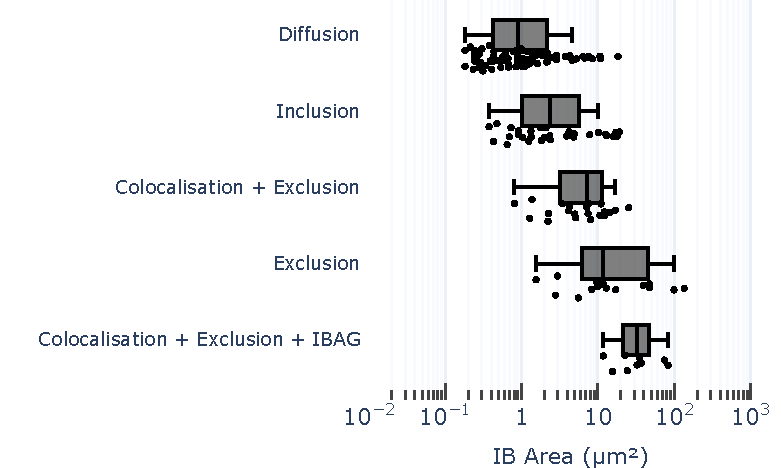
\includegraphics[width=1\linewidth]{09. Chapter 4/Figs/02. Overexpression/02. IFIT2/02. box_hi2f_hrsv.pdf}
    \end{subfigure}
    \caption[Observed Phenotypes of Exogenous hIFIT2 in the Context of hRSV Inclusion Bodies in Vero Cell Line.]{\textbf{Observed Phenotypes of Exogenous hIFIT2 in the Context of hRSV Inclusion Bodies in Vero Cell Line.} Vero cells were infected with human RSV at MOI 1. 24 HPI, the cells were transfected with hIFIT2-FLAG containing plasmids using TransIT-X2 and were fixed after a further 24 hours. Cells were labelled with anti-RSV N and anti-FLAG antibodies and imaged on a confocal microscope. Panel (a) shows the percentual proportions of observed phenotypes between hRSV inclusion bodies and exogenous hIFIT2 (155 observations), with the red dotted line denoting the 5\% threshold, marking phenotypes considered relevant above this limit. Panel (b) shows the IB area in \(\mu \mbox{m}^2\) per observed relevant phenotype.}
    \label{fig:Observed Phenotypes of Exogenous hIFIT2 in the Context of hRSV Inclusion Bodies in Vero Cell Line}
\end{figure}

\begin{figure}
    \centering
    \includegraphics[width=1\linewidth]{09. Chapter 4/Figs/02. Overexpression/02. IFIT2/03. hi2f-hrsv.pdf}
    \caption[Representative Images of Observed Phenotypes of Exogenous hIFIT2 in the Context of hRSV Inclusion Bodies in Vero Cell Line.]{\textbf{Representative Images of Observed Phenotypes of Exogenous hIFIT2 in the Context of hRSV Inclusion Bodies in Vero Cell Line.} Vero cells were infected with human RSV at MOI 1. 24 HPI, the cells were transfected with hIFIT2-FLAG containing plasmids using TransIT-X2 and were fixed after a further 24 hours. Cellular nuclei were stained with DAPI (yellow), and cells were double-labelled with anti-RSV N (cyan) and anti-FLAG (magenta) antibodies. This figure showcases representative examples of relevant phenotypes in the interaction between exogenous hIFIT2 and hRSV inclusion bodies. These phenotypes are presented in descending order based on their percentage proportions. The scale bar indicates 2 \(\mu \mbox{m}\).}
    \label{fig:Representative Images of Observed Phenotypes of Exogenous hIFIT2 in the Context of hRSV Inclusion Bodies in Vero Cell Line}
\end{figure}

Next we set to validate the data obtained from exopgenbously expressed human and bovine IFT2-FLAG in the context of human or bovine RSV pIBs by inducing the expression of human and bovine IFIT2-FLAG in hRSV and bRSV infected cells. The experimental methodology follows what was described Section \ref{subsec:Overexpressed IFIT1, IFIT3, and IFIT5 During RSV Infection}. In short Vero cells were initially infected with either human or bovine RSV at MOI 1 according to the standard protocol. 24 HPI the cells were transfected with either human or bovine IFIT2-FLAG containing plasmid and were fixed after further 24 hours. 

Initially we looked at the interaction phenotypes of exogenously expressed human IFIT2-FLAG with hRSV inclusion bodies. We have obtained 155 observations. The frequencies of the observed phenotypes along with the IB sizes detected poer phenotypes that occured with higher than 5\% frequency are shown in FIgure \ref{fig:Observed Phenotypes of Exogenous hIFIT2 in the Context of hRSV Inclusion Bodies in Vero Cell Line}. The representative images of the latter are shown in Figure \ref{fig:Representative Images of Observed Phenotypes of Exogenous hIFIT2 in the Context of hRSV Inclusion Bodies in Vero Cell Line}. We have observed a diverse range of interaction phenotypes. The most commonly occuring was diffusion phuenotype, whioch occured in 48\% of all observartions. This was followed by inclusion (22\%), colocalisation associated with exclusion (14\%), exclusion (9\%), and cplpcalsation of IFIT2 with the IB boundry, while being excluded from the middle with the exeption of IFIT2 spots, which resembeled IBAGs (5\% of all observations). We have also observed colocalsation phenotype and exclusion associated with the presence of IFIT2 spots within the IB boundry, both of which only appeared in 1\% of observations and thus were not part ofthe IB size analysis. With regards to the size of the IBs assocated with the different phenotypes, we can observe a clear size separation based on the median IB size, although there is size overlap between phenotypes. The diffusion phenotype occured predominantly in smaller, sub 1 \(\mu \mbox{m}^2\) IBs, although it was detected also in medium siozed and large IBs (size range from 0.18 \(\mu \mbox{m}^2\) to 19 \(\mu \mbox{m}^2\), with the typical size of 0.9 \(\mu \mbox{m}^2\)). The range of sizes of inbclusion-associated IBs is contained within the range of diffusion-associated IBs, however the median value of the former is larger. In more detail, the inlucion associated IBs ranged from 0.37 \(\mu \mbox{m}^2\) to 19 \(\mu \mbox{m}^2\), with a median value of 2.1 \(\mu \mbox{m}^2\). The colocalisation associated with exclusion occured in IBs raging from 0.8 \(\mu \mbox{m}^2\) to 25 \(\mu \mbox{m}^2\), with the median value of 7 \(\mu \mbox{m}^2\). We have observed the exclusion phenotype to occur in IBs ranging from 1.5 \(\mu \mbox{m}^2\) to 130 \(\mu \mbox{m}^2\), with the median size of 11 \(\mu \mbox{m}^2\). These IBs often showed a discint morphology compared to IBs associated with other phenotypes (Figure \ref{fig:Representative Images of Observed Phenotypes of Exogenous hIFIT2 in the Context of hRSV Inclusion Bodies in Vero Cell Line}), which we think are inclusion bodies that are undergoing degradation. Lastly, we observed cplpcalsation of IFIT2 with the IB boundry, while being excluded from the middle with the exeption of IFIT2 spots to occur in very large IBs, ranging fdrom 11 \(\mu \mbox{m}^2\) to 83 \(\mu \mbox{m}^2\), with the median size of 32 \(\mu \mbox{m}^2\).

This means that IFIT2 is associated with small (sub 1 \(\mu \mbox{m}^2\)) via predominantly diffusion and occuasionaly forming inclusions, while the medium sized IBs (between 1 \(\mu \mbox{m}^2\) and 10 \(\mu \mbox{m}^2\)) confront to diffusion,inclusion, and colocalisation associated with exclusion phenotypes. Large IBs (above 10 \(\mu \mbox{m}^2\)) have the propensity to confront to all phenotipic interactions, but as their size increases the predominant interaction phenotypes become colocalisationa associated with exclusion (with or without spots) and the exclusion phenotype. From the literature we know that as IBs increase in size, they mature, increase in complexity (e.g. appearence of IBAGs), and their stucture befomes more gel like \cite{Weber1995NonstructuralSerum, Fricke2013P38Assembly, Rincheval2017FunctionalVirus, Jobe2021BovineResponses}. This suggest that the interaction of exogenous human IFIT2 with hRSV inclusion bodies depends on their maturation level. Along to this, this data shows that IFIT2 exhibits approximately equal frequency of phenotypes that are suggesting IB interaction (inclusion and colocalisation) to the ones tham imply no or minimal interaction (diffusion and exclusion). Overall thise data replicate what was observed with endogenous human and bovine IFIT2s during RSV infection, or human and monkey IFIT2 with the context of RSV pIBs, if we assume that IFIT2(A) and IFIT2(B) antibodies collectively detect the whole IFIT2 population.

\begin{figure}
    \begin{subfigure}{0.495\textwidth}
        \caption{}
        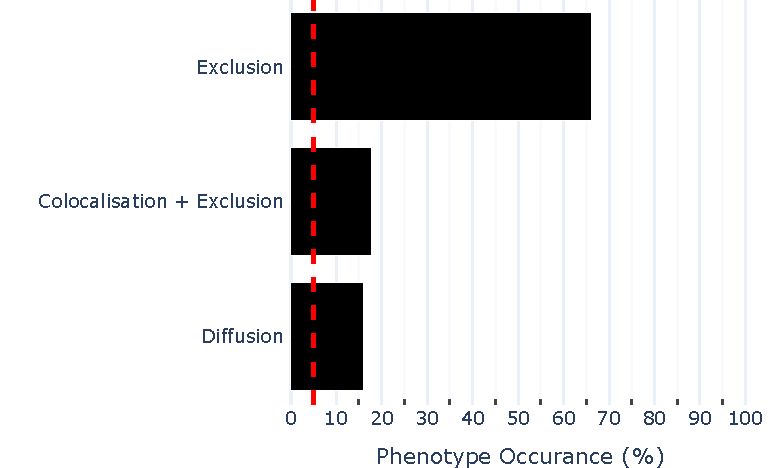
\includegraphics[width=1\linewidth]{09. Chapter 4/Figs/02. Overexpression/02. IFIT2/04. bar_bi2f_hrsv.pdf} 
    \end{subfigure}
    \begin{subfigure}{0.495\textwidth}
        \caption{}
        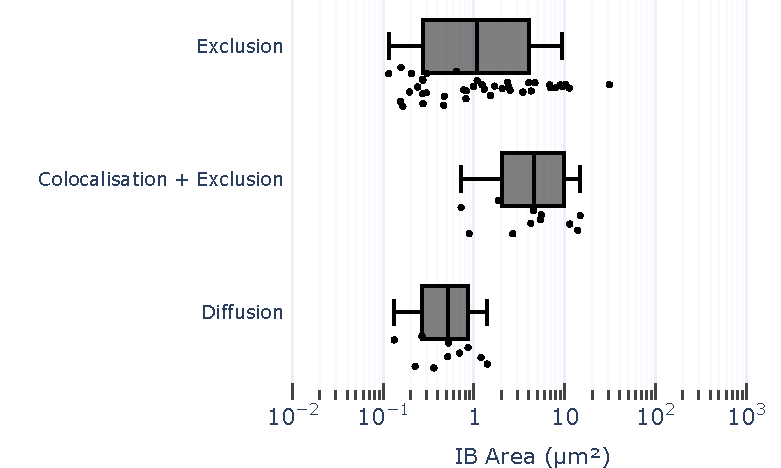
\includegraphics[width=1\linewidth]{09. Chapter 4/Figs/02. Overexpression/02. IFIT2/05. box_bi2f_hrsv.pdf}
    \end{subfigure}
    \caption[Observed Phenotypes of Exogenous bIFIT2 in the Context of hRSV Inclusion Bodies in Vero Cell Line.]{\textbf{Observed Phenotypes of Exogenous bIFIT2 in the Context of hRSV Inclusion Bodies in Vero Cell Line.} Vero cells were infected with human RSV at MOI 1. 24 HPI, the cells were transfected with bIFIT2-FLAG containing plasmids using TransIT-X2 and were fixed after a further 24 hours. Cells were labelled with anti-RSV N and anti-FLAG antibodies and imaged on a confocal microscope. Panel (a) shows the percentual proportions of observed phenotypes between hRSV inclusion bodies and exogenous bIFIT2 (62 observations), with the red dotted line denoting the 5\% threshold, marking phenotypes considered relevant above this limit. Panel (b) shows the IB area in \(\mu \mbox{m}^2\) per observed relevant phenotype.}
    \label{fig:Observed Phenotypes of Exogenous bIFIT2 in the Context of hRSV Inclusion Bodies in Vero Cell Line}
\end{figure}

\begin{figure}
    \centering
    \includegraphics[width=1\linewidth]{09. Chapter 4/Figs/02. Overexpression/02. IFIT2/06. bi2f-hrsv.pdf}
    \caption[Representative Images of Observed Phenotypes of Exogenous bIFIT2 in the Context of hRSV Inclusion Bodies in Vero Cell Line.]{\textbf{Representative Images of Observed Phenotypes of Exogenous bIFIT2 in the Context of hRSV Inclusion Bodies in Vero Cell Line.} Vero cells were infected with human RSV at MOI 1. 24 HPI, the cells were transfected with bIFIT2-FLAG containing plasmids using TransIT-X2 and were fixed after a further 24 hours. Cellular nuclei were stained with DAPI (yellow), and cells were double-labelled with anti-RSV N (cyan) and anti-FLAG (magenta) antibodies. This figure showcases representative examples of relevant phenotypes in the interaction between exogenous bIFIT2 and hRSV inclusion bodies. These phenotypes are presented in descending order based on their percentage proportions. The scale bar indicates 2 \(\mu \mbox{m}\).}
    \label{fig:Representative Images of Observed Phenotypes of Exogenous bIFIT2 in the Context of hRSV Inclusion Bodies in Vero Cell Line}
\end{figure}

Next, we set to investigate the exogenously expressed human IFIT2-FLAG and its interaction with bRSV inclusion bodies, however, we failed to observe a single co-infected/transfect cells after many attempts. Due to this we have shifted our focus on exogenously expressed bovine IFIT2-FLAG and its localisation with hRSV IBs. Within the 62 detected bIFIT2/hRSV IB interactions, we have observed 3 interaction phenotypes. Their frequencies of occurances along with the IB sizes per phenotype are shown in Figure \ref{fig:Observed Phenotypes of Exogenous bIFIT2 in the Context of hRSV Inclusion Bodies in Vero Cell Line}. The representative images of these bIFIT2/hRSV IB interactions are shown in Figure \ref{fig:Representative Images of Observed Phenotypes of Exogenous bIFIT2 in the Context of hRSV Inclusion Bodies in Vero Cell Line}. The most comonly occuring intreraction phenotype was exlusion, which occured in 66\% of observations. The sizes of IBs associated with this phenotypes spanned the whole IB size spectrum, ranging from 0.11 \(\mu \mbox{m}^2\) to 30 \(\mu \mbox{m}^2\), with the typical size of 1 \(\mu \mbox{m}^2\). Next most frequent phenotype was colocalisation associated with exclusion, which was observed in 17\% of all observations. This phenotype predominantly occured in larger IBs, ranging in size from 0.7 \(\mu \mbox{m}^2\) to 15 \(\mu \mbox{m}^2\), with the median size of 5 \(\mu \mbox{m}^2\). Lastly, we have observed bIFIT2 to be diffusied equally between the cytoplasm and IB nstructures in 16\% of the obsaervations. The diffusion-associated IBs were of smaller size, ranging from 0.12 \(\mu \mbox{m}^2\) to 1.3 \(\mu \mbox{m}^2\), with the mnedian value of 0.55 \(\mu \mbox{m}^2\). Overall, we can see that the exclusion phenotype occurs most commonly and across the whole size spectrum. The reimaining third of bIFIT2-FRSV IB interactions was almost equally divided between colocalisation associated with exclusion, and diffusion phenotype. These occured in size specific manner.

\begin{figure}
    \begin{subfigure}{0.495\textwidth}
        \caption{}
        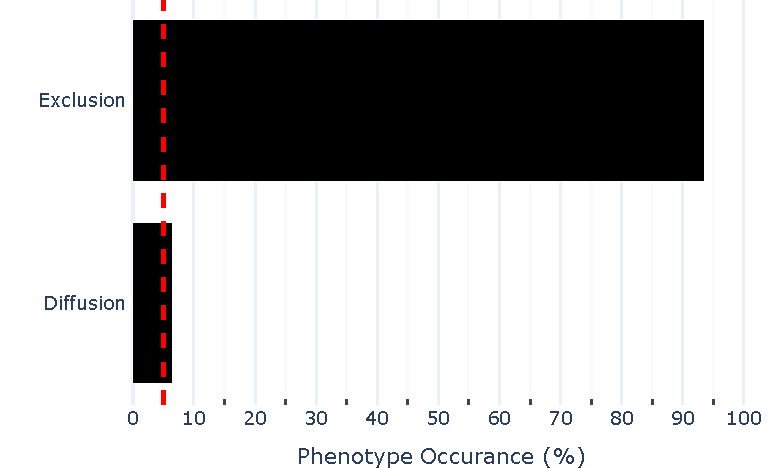
\includegraphics[width=1\linewidth]{09. Chapter 4/Figs/02. Overexpression/02. IFIT2/07. bar_bi2f_brsv.pdf} 
    \end{subfigure}
    \begin{subfigure}{0.495\textwidth}
        \caption{}
        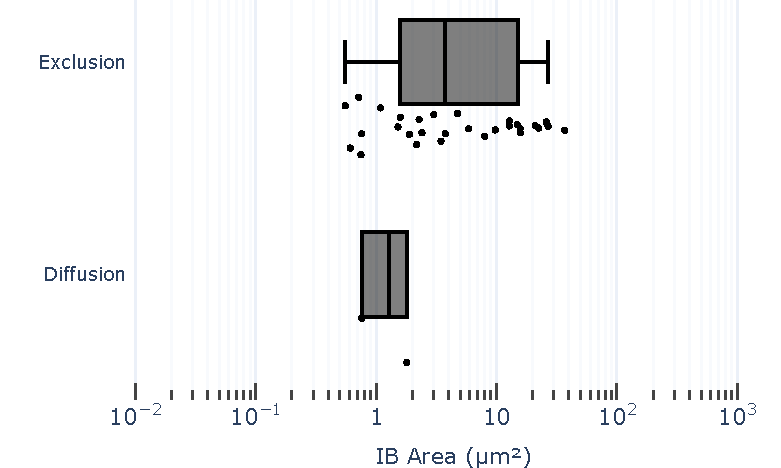
\includegraphics[width=1\linewidth]{09. Chapter 4/Figs/02. Overexpression/02. IFIT2/08. box_bi2f_brsv.pdf}
    \end{subfigure}
    \caption[Observed Phenotypes of Exogenous bIFIT2 in the Context of bRSV Inclusion Bodies in Vero Cell Line.]{\textbf{Observed Phenotypes of Exogenous bIFIT2 in the Context of bRSV Inclusion Bodies in Vero Cell Line.} Vero cells were infected with human RSV at MOI 1. 24 HPI, the cells were transfected with bIFIT2-FLAG containing plasmids using TransIT-X2 and were fixed after a further 24 hours. Cells were labelled with anti-RSV N and anti-FLAG antibodies and imaged on a confocal microscope. Panel (a) shows the percentual proportions of observed phenotypes between bRSV inclusion bodies and exogenous bIFIT2 (31 observations), with the red dotted line denoting the 5\% threshold, marking phenotypes considered relevant above this limit. Panel (b) shows the IB area in \(\mu \mbox{m}^2\) per observed relevant phenotype.}
    \label{fig:Observed Phenotypes of Exogenous bIFIT2 in the Context of bRSV Inclusion Bodies in Vero Cell Line}
\end{figure}

\begin{figure}
    \centering
    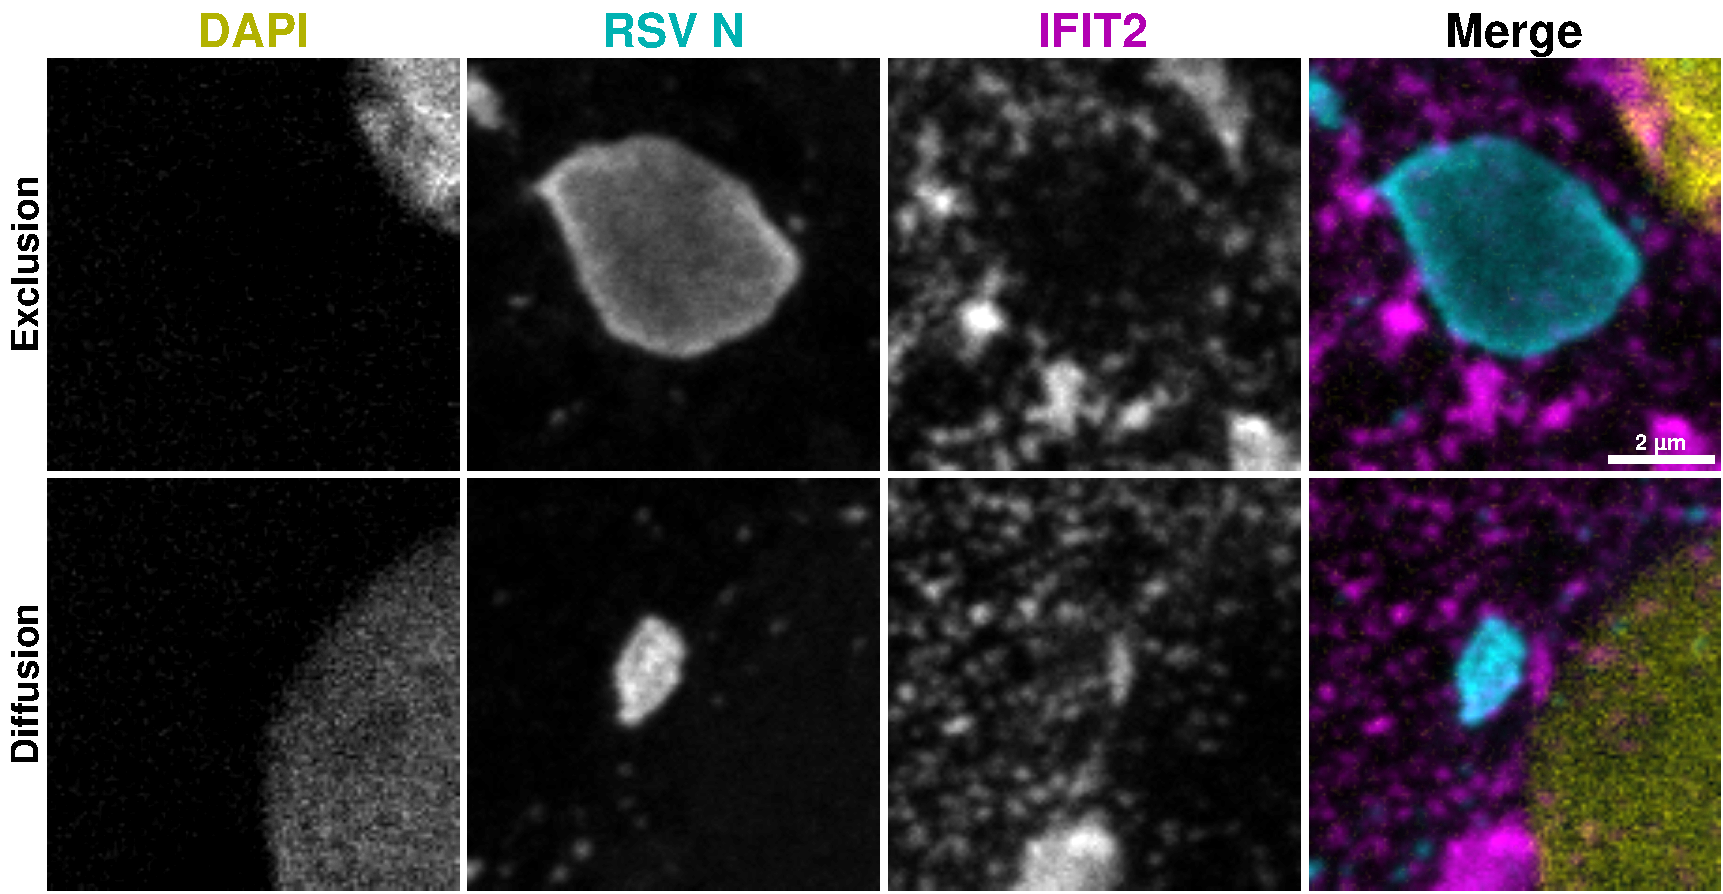
\includegraphics[width=1\linewidth]{09. Chapter 4/Figs/02. Overexpression/02. IFIT2/09. bi2f-brsv.pdf}
    \caption[Representative Images of Observed Phenotypes of Exogenous bIFIT2 in the Context of bRSV Inclusion Bodies in Vero Cell Line.]{\textbf{Representative Images of Observed Phenotypes of Exogenous bIFIT2 in the Context of bRSV Inclusion Bodies in Vero Cell Line.} Vero cells were infected with human RSV at MOI 1. 24 HPI, the cells were transfected with bIFIT2-FLAG containing plasmids using TransIT-X2 and were fixed after a further 24 hours. Cellular nuclei were stained with DAPI (yellow), and cells were double-labelled with anti-RSV N (cyan) and anti-FLAG (magenta) antibodies. This figure showcases representative examples of relevant phenotypes in the interaction between exogenous bIFIT2 and bRSV inclusion bodies. These phenotypes are presented in descending order based on their percentage proportions. The scale bar indicates 2 \(\mu \mbox{m}\).}
    \label{fig:Representative Images of Observed Phenotypes of Exogenous bIFIT2 in the Context of bRSV Inclusion Bodies in Vero Cell Line}
\end{figure}

Finally, we have investigated the interaction of exogenously expressed bovine IFIT2-FLAG with bRSV inclusion bodies. We have obtained 31 IB/bIFIT2 interaction observations. The frequencies of the interaction observed intraction phenotypes, along with the IB sizes assocated with these phenotypes is shown in Figure \ref{fig:Observed Phenotypes of Exogenous bIFIT2 in the Context of bRSV Inclusion Bodies in Vero Cell Line}. The representative images of these phenotypes are shown in Figure \ref{fig:Representative Images of Observed Phenotypes of Exogenous bIFIT2 in the Context of bRSV Inclusion Bodies in Vero Cell Line}. In the majority of cases (94\%) we have observed exogenous bIFIT2 to be excluded from bRSV IBs. These occured in both small and large IBs, which ranged from 0.54 \(\mu \mbox{m}^2\) to 37 \(\mu \mbox{m}^2\), with a atypical size of 3.9 \(\mu \mbox{m}^2\). We also obtained two obsevations of diffusion phenotype which were 0.8 \(\mu \mbox{m}^2\) and 1.8 \(\mu \mbox{m}^2\) in size. ...

94 6

0.54 3.9 37
0.8 1.8

maybe if more large ones we would see coloc + excl

summary

paragraph of putting infection and all 2 together

prepare for rbm - positive interaction could be mediated via i2-rna interaction

\subsection{Endeavour in Understanding the Mechanisms of IFIT2-RSV IB Interaction} \label{subsec:Endeavour in Understanding the Mechanisms of IFIT2-RSV IB Interaction}
%The Generation of Bovine IFIT2 RNA-Binding Mutant
Using published data about hIFIT2 rna-binding mutant

Difficulty of using alpha-fold with IFIT2 due to the swap domain

Using SWISS-MODEL to predict bIFIT2 structure from published hIFIT2 structures

Alignment of both structures, assessment of electrostatic charges and establishment of residues to be mutated

Primer design and mutagenesis procedure based on published hIFIT2 RNA-binding mutant paper
\cite{Tran2020InfluenzaMRNAs}

\ref{subsec:PCR for Point Mutant Generation}

\begin{figure}
    \centering
    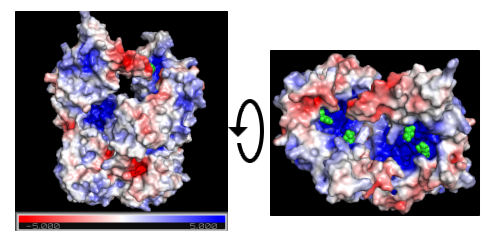
\includegraphics[width=1\linewidth]{09. Chapter 4/Figs/01. pIB/03. IFIT2/05. IFIT2-RNA binding mutant/01. Structure/01. structure.png}
    \caption[ifit2 mutant structure]{\textbf{bifit2 mutant structure.} write caption}
    \label{fig:ifit2 mutant structure}
\end{figure}






\begin{figure}
    \begin{subfigure}{0.495\textwidth}
        \caption{}
        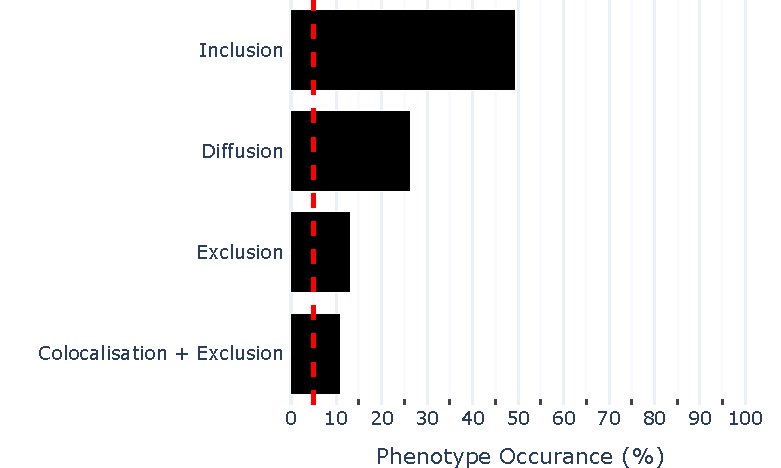
\includegraphics[width=1\linewidth]{09. Chapter 4/Figs/01. pIB/03. IFIT2/05. IFIT2-RNA binding mutant/02. pIB/01. bar_bi2f24_hnhp.pdf} 
    \end{subfigure}
    \begin{subfigure}{0.495\textwidth}
        \caption{}
        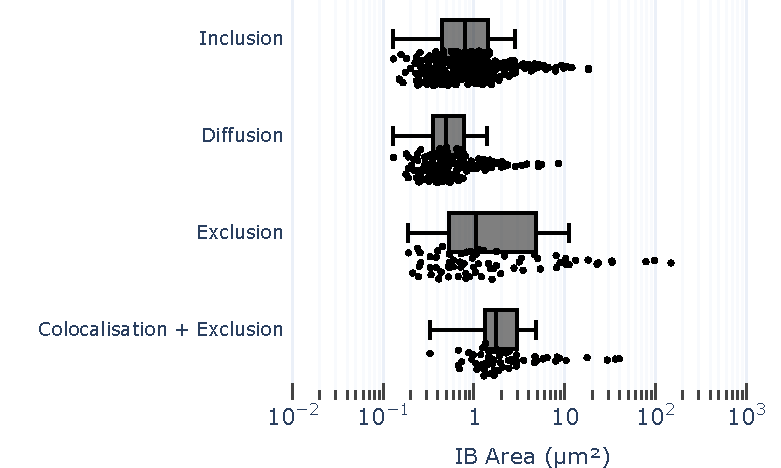
\includegraphics[width=1\linewidth]{09. Chapter 4/Figs/01. pIB/03. IFIT2/05. IFIT2-RNA binding mutant/02. pIB/02. box_bi2f24_hnhp.pdf}
    \end{subfigure}
    \caption[Diverse Phenotypic Interactions of Bovine IFIT2 RNA-Binding Mutant with Human RSV Pseudo Inclusion Bodies (pIBs) in the Vero Cell Line.]{\textbf{Diverse Phenotypic Interactions of Bovine IFIT2 RNA-Binding Mutant with Human RSV Pseudo Inclusion Bodies (pIBs) in the Vero Cell Line.} Vero cells were transfected with hRSV N and P, along with bovine IFIT2-FLAG RNA-binding mutant containing plasmids using TransIT-X2 and were fixed after 24 hours. Cells were labelled with anti-RSV N and anti-FLAG antibodies and imaged on a confocal microscope. Panel (a) shows percentual proportions of observed phenotypes between hRSV pseudo inclusion bodies and exogenous bovine IFIT2-FLAG RNA-binding mutant (548 observations), with the red dotted line denoting the 5\% threshold, marking phenotypes considered relevant above this limit. Panel (b) shows the IB area in \(\mu \mbox{m}^2\) per observed relevant phenotype.}
    \label{fig:Diverse Phenotypic Interactions of Bovine IFIT2 RNA-Binding Mutant with Human RSV Pseudo Inclusion Bodies (pIBs) in the Vero Cell Line}
\end{figure}

\begin{figure}
    \centering
    \includegraphics[width=1\linewidth]{09. Chapter 4/Figs/01. pIB/03. IFIT2/05. IFIT2-RNA binding mutant/02. pIB/03. bi2f24-hnhp.pdf}
    \caption[Representative Images of Diverse Phenotypic Interactions of Bovine IFIT2 RNA-Binding Mutant with Human RSV Pseudo Inclusion Bodies (pIBs) in the Vero Cell Line.]{\textbf{Representative Images of Diverse Phenotypic Interactions of Bovine IFIT2 RNA-Binding Mutant with Human RSV Pseudo Inclusion Bodies (pIBs) in the Vero Cell Line.}  Vero cells were transfected with bRSV N and P, along with bovine IFIT2-FLAG RNA-binding mutant containing plasmids using TransIT-X2 and were fixed after 24 hours. Cellular nuclei were stained with DAPI (yellow), and cells were double-labelled with anti-RSV N (cyan) and anti-FLAG (magenta) antibodies. This figure showcases representative examples of relevant phenotypes in the interaction between exogenous bovine IFIT2-FLAG RNA-binding mutant and hRSV pseudo-inclusion bodies. These phenotypes are presented in descending order based on their percentage proportions. The scale bar indicates 2 \(\mu \mbox{m}\).}
    \label{fig:Representative Images of Diverse Phenotypic Interactions of Bovine IFIT2 RNA-Binding Mutant with Human RSV Pseudo Inclusion Bodies (pIBs) in the Vero Cell Line}
\end{figure}

49 27 13 11

0.12 0.8 19
0.12 0.5 8.5
0.19 1 140
0.31 1.8 40

\begin{figure}
    \begin{subfigure}{0.495\textwidth}
        \caption{}
        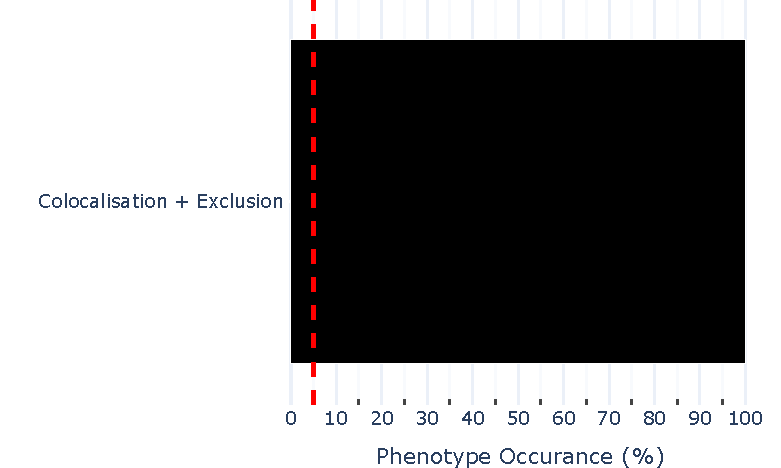
\includegraphics[width=1\linewidth]{09. Chapter 4/Figs/01. pIB/03. IFIT2/05. IFIT2-RNA binding mutant/02. pIB/04. bar_bi2f24_bnbp.pdf} 
    \end{subfigure}
    \begin{subfigure}{0.495\textwidth}
        \caption{}
        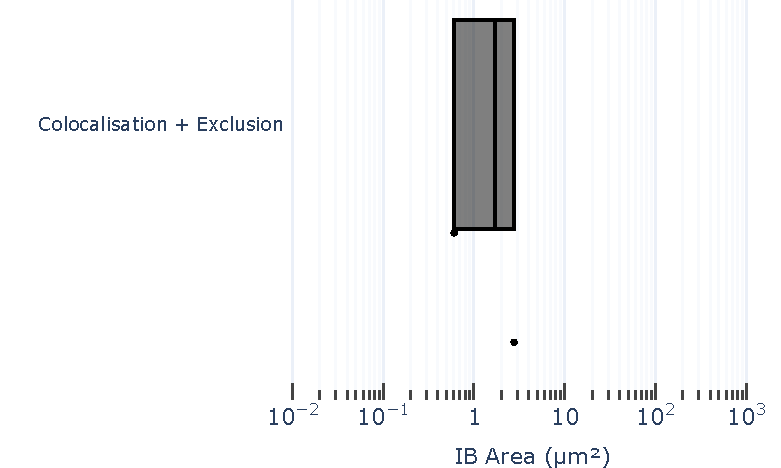
\includegraphics[width=1\linewidth]{09. Chapter 4/Figs/01. pIB/03. IFIT2/05. IFIT2-RNA binding mutant/02. pIB/05. box_bi2f24_bnbp.pdf}
    \end{subfigure}
    \caption[Diverse Phenotypic Interactions of Bovine IFIT2 RNA-Binding Mutant with Bovine RSV Pseudo Inclusion Bodies (pIBs) in the Vero Cell Line.]{\textbf{Diverse Phenotypic Interactions of Bovine IFIT2 RNA-Binding Mutant with Bovine RSV Pseudo Inclusion Bodies (pIBs) in the Vero Cell Line.} Vero cells were transfected with bRSV N and P, along with bovine IFIT2-FLAG RNA-binding mutant containing plasmids using TransIT-X2 and were fixed after 24 hours. Cells were labelled with anti-RSV N and anti-FLAG antibodies and imaged on a confocal microscope. Panel (a) shows percentual proportions of observed phenotypes between bRSV pseudo inclusion bodies and exogenous bovine IFIT2-FLAG RNA-binding mutant (2 observations), with the red dotted line denoting the 5\% threshold, marking phenotypes considered relevant above this limit. Panel (b) shows the IB area in \(\mu \mbox{m}^2\) per observed relevant phenotype.}
    \label{fig:Diverse Phenotypic Interactions of Bovine IFIT2 RNA-Binding Mutant with Bovine RSV Pseudo Inclusion Bodies (pIBs) in the Vero Cell Line}
\end{figure}

\begin{figure}
    \centering
    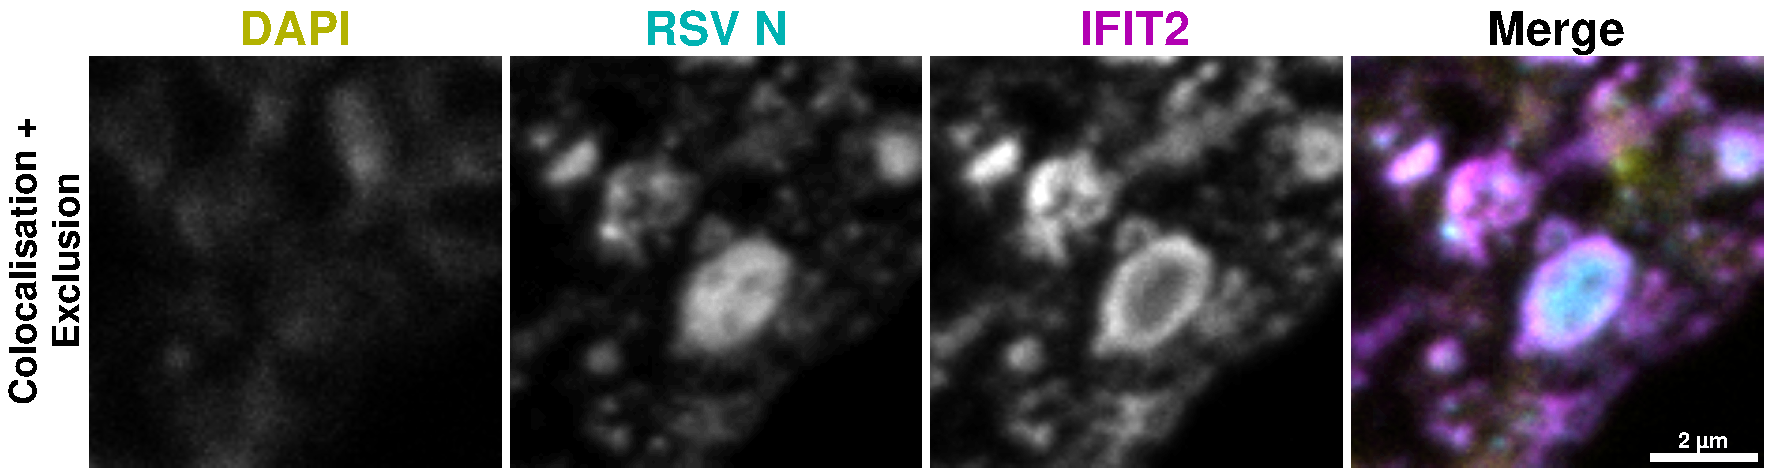
\includegraphics[width=1\linewidth]{09. Chapter 4/Figs/01. pIB/03. IFIT2/05. IFIT2-RNA binding mutant/02. pIB/06. bi2f24-bnbp.pdf}
    \caption[Representative Images of Diverse Phenotypic Interactions of Bovine IFIT2 RNA-Binding Mutant with Bovine RSV Pseudo Inclusion Bodies (pIBs) in the Vero Cell Line.]{\textbf{Representative Images of Diverse Phenotypic Interactions of Bovine IFIT2 RNA-Binding Mutant with Bovine RSV Pseudo Inclusion Bodies (pIBs) in the Vero Cell Line.}  Vero cells were transfected with bRSV N and P, along with bovine IFIT2-FLAG RNA-binding mutant containing plasmids using TransIT-X2 and were fixed after 24 hours. Cellular nuclei were stained with DAPI (yellow), and cells were double-labelled with anti-RSV N (cyan) and anti-FLAG (magenta) antibodies. This figure showcases representative examples of relevant phenotypes in the interaction between exogenous bovine IFIT2-FLAG RNA-binding mutant and bRSV pseudo inclusion bodies. These phenotypes are presented in descending order based on their percentage proportions. The scale bar indicates 2 \(\mu \mbox{m}\).}
    \label{fig:Representative Images of Diverse Phenotypic Interactions of Bovine IFIT2 RNA-Binding Mutant with Bovine RSV Pseudo Inclusion Bodies (pIBs) in the Vero Cell Line}
\end{figure}

100

0.6 2.9


transfecting bi2f24 + bngfp + p inhibits bpIBs (compared to hi2f or bi2f)

% summary i2
We have described how bovine IFIT2 RNA-binding mutant was designed based on the published human IFIT2 RNA-binding mutant data (needs to be annotated more). Overexpression of bovine IFIT2 RNA-binding mutant yields cellular distribution and morphology similar to what was observed with overexpressing human IFIT2-FLAG, suggesting that the mutant proteins are not toxic to the cells. In the first experiment where we were looking at interaction between bovine IFIT2 RNA-binding mutant and human pseudo inclusion bodies we saw several phenotypes. We observed bovine IFIT2 RNA-binding mutant being excluded from small and big pIBs and pIB associated filamentous network, while fully or partially colocalising with other pIBs. In a subsequent experiment we observed only colocalization and inclusion formation. When assessing the interaction between bovine IFIT2 RNA-binding mutant and human pIBs formed using wild-type human RSV P and GFP-tagged human RSV N, we observed consistently in two experiments that bovine IFIT2 RNA-binding mutant colocalises to the pIB structures.